\documentclass[aspectratio=169,9pt,handout]{beamer}

%\transdissolve[duration=0.2] % Only works with Adobe Acrobat

% Some important packages
\usepackage{epstopdf}
\usepackage{ulem} % sout
\hypersetup{colorlinks=false, allcolors=purple}
\usepackage{booktabs}
\linespread{1.3}
\usepackage{tabularx,multirow}
\usepackage{makecell} % For makecell within tables
\usepackage{geometry}
\usepackage{fancybox}
\usepackage{algorithm2e}
\usepackage{amsmath, amssymb}
% Mathematical functions
% DELETED!
\renewcommand{\Pr}[1]{{\mathbb{P}\left(#1\right) }}
% DELETED!
% DELETED!
% DELETED!
% DELETED!
% DELETED!

% DELETED!
\newcommand{\sufstats}[1]{s\left(#1\right)}
\renewcommand{\exp}[1]{\mbox{exp}\left\{#1\right\}}
\renewcommand{\log}[1]{\mbox{log}\left\{#1\right\}}
\newcommand{\transpose}[1]{{#1}^\mathbf{t}}
\renewcommand{\t}[1]{\transpose{#1}}

\newcommand{\s}[1]{\sufstats{#1}}
\newcommand{\SUFF}{\mathcal{S}}
\newcommand{\Suff}{\mathbf{S}}
\newcommand{\suff}{\mathbf{s}}

\renewcommand{\beta}{\theta}
\newcommand{\weight}{\mathbf{w}}
\newcommand{\Weight}{\mathbf{W}}

% Objects
% DELETED!
% DELETED!
\newcommand{\Graph}{\mathbf{G}}
\newcommand{\graph}{\mathbf{g}}
\newcommand{\GRAPH}{\mathcal{G}}
\newcommand{\Adjmat}{Y}
\newcommand{\adjmat}{y}
\newcommand{\ADJMAT}{\mathcal{Y}}

\newcommand{\INDEPVAR}{\mathcal{X}}
\newcommand{\Indepvar}{X}
\newcommand{\indepvar}{x}

\newcommand{\normconst}{\kappa\left(\params, \Indepvar\right)}

\graphicspath{{./figures/}{.}{./terms/}}


%% NEED THIS FOR CANCY TEX
\usepackage{pstricks}

% Colors
\definecolor{USCCardinal}{HTML}{990000} % 153 0 0 in RGB
\definecolor{USCGold}{HTML}{FFCC00}
\definecolor{USCGray}{HTML}{CCCCCC}

% \bibliography{bibliography.bib}

\def\ergmito{ERGM\textit{ito}}
\def\ergmitos{\ergmito{}\textit{s}}
% Mathematical functions
\newcommand{\isone}[1]{{\boldsymbol{1}\left( #1 \right)}}
\renewcommand{\Pr}[1]{{\mathbb{P}\left(#1\right) }}
\newcommand{\f}[1]{{f\left(#1\right) }}
\newcommand{\Prcond}[2]{{\mathbb{P}\left(#1\vphantom{#2}\;\right|\left.\vphantom{#1}#2\right)}}
\newcommand{\fcond}[2]{{f\left(#1|#2\right) }}
\newcommand{\Expected}[1]{{\mathbb{E}\left\{#1\right\}}}
\newcommand{\ExpectedCond}[2]{{\mathbb{E}\left\{#1\vphantom{#2}\right|\left.\vphantom{#1}#2\right\}}}
\renewcommand{\exp}[1]{\mbox{exp}\left\{#1\right\}}

\newcommand{\Likelihood}[2]{\text{L}\left(#1 \left|\vphantom{#1}#2\right.\right)}

\newcommand{\loglik}[1]{l\left(#1\right)}


% Mathematical Annotation -------------------------------
% Modify this so that it matches the P01 convention overall

% Tree
\newcommand{\phylo}{\Lambda{}} % The actual tree
\newcommand{\aphylo}{D{}}      % The annotated phylogenetic tree
\newcommand{\aphyloObs}{\tilde \aphylo{}} % The observed annotated phylogenetic tree
\newcommand{\parent}[1]{\mathbf{p}\left(#1\right)}
\newcommand{\offspring}[1]{\mathbf{O}\left(#1\right)}
\newcommand{\nodes}{\mathcal{N}{}}
\newcommand{\edges}{\mathcal{E}{}}

\newcommand{\class}[1]{C_{#1}{}}

% Annotations
\newcommand{\Ann}{\mathbf{X}{}} % Matrix of "real" annotations
\newcommand{\ann}[1]{x_{#1}{}} % single element of "real" annotations
\newcommand{\constraints}{\mathcal{C}{}} % Taxon constraints

% Obs Annotations
\newcommand{\AnnObs}{\mathbf{Z}{}}%{Z{}} \mathbf{X}^{obs}{}
\newcommand{\annObs}[1]{z_{#1}{}}%{z{}}  x_{#1}^{obs

% Pred. Annotations
\newcommand{\AnnPred}{\hat X{}}
\newcommand{\annPred}[1]{\hat x_{#1}}

% Leaf nodes
\newcommand{\Leaf}{L{}}

% Shortest path
\newcommand{\Geodesic}{\text{T}{}}
\newcommand{\geodesic}{\tau{}}

\newcommand{\Params}{\Omega{}}
\newcommand{\params}{\omega{}}

% Parameters
\newcommand{\gain}{\mu_{01}{}}
\newcommand{\loss}{\mu_{10}{}}
\newcommand{\misszero}{\psi_{01}{}}
\newcommand{\missone}{\psi_{10}{}}
\newcommand{\proot}{\pi}


% New notation ------------------------------------------------------------------
\newcommand{\expo}{E}
\newcommand{\Expo}{\mathbf{\expo{}}}
\newcommand{\expod}[1]{\expo_{#1}^D}
\newcommand{\expoc}[1]{\expo_{#1}^C}
\newcommand{\expoi}[1]{\expo_{#1}^I}

\newcommand{\covar}{\mathbf{x}}
\newcommand{\Covar}{\mathbf{X}}
\newcommand{\latent}{\mathbf{z}}
\newcommand{\Latent}{\mathbf{z}}

\newcommand{\Event}{\mbox{P}}
\newcommand{\pset}[1]{\mathcal{P}\left(#1\right)}
\newcommand{\size}[1]{\left|#1\right|}

\newcommand{\logit}[1]{\mbox{logit}^{-1}\left(#1\right)}
% -------------------------------------------------------------------------------

\usepackage[style=authoryear-comp]{biblatex}
\addbibresource{bibliography-aphylo.bib}
\addbibresource{bibliography-ergmito.bib}
\addbibresource{bibliography-extra.bib}
\addbibresource{bibliography.bib}
% \renewcommand{\bibsection}{\subsubsection*{\bibname } }

% Neat trick to change the mode mid-presentation
% https://tex.stackexchange.com/questions/91691/beamer-set-mode-mid-presentation?rq=1
\makeatletter
\newcommand\changemode[1]{%
	\gdef\beamer@currentmode{#1}}
\makeatother


% Styles
\usepackage{xcolor}
\usepackage{colortbl}
\definecolor{suffstat}{RGB}{10,159,0}
\definecolor{normconst}{RGB}{87,38,231}
\setbeamercolor{conclusions}{bg=usclightgray!60!white, fg=uscdarkgray}

% Noice!
\usetheme{usckeck}

\title[Stat. Comp. for Complex Systems]{%
	Statistical and Computational Methods for Complex Systems
}
\author[GGVY -- \href{vegayon@usc.edu}{vegayon@usc.edu}]{George G Vega Yon}
\institute[USC-PREVMED]{University of Southern California, Department of Preventive Medicine}
\date{Universidad Adolfo Ibáñez\\December 10, 2020}

% Some definitions
\def\cursection{\frame{\frametitle{Contents}\tableofcontents[current]}}
\newcommand{\ergmpkg}[0]{\texttt{ergm}}
\newcommand{\ergmitopkg}[0]{\texttt{ergmito}}
\newcommand{\aphylopkg}[0]{\texttt{aphylo}}
\graphicspath{{.}{fig/}{fig-whoami/}{fig-struct-test/}}

\usepackage{media9}


% ------------------------------------------------------------------------------
% ------------------------------------------------------------------------------
% --------------------------- END OF PREAMBLE ----------------------------------
% ------------------------------------------------------------------------------
% ------------------------------------------------------------------------------
\setbeamertemplate{note page}[plain]
%\setbeameroption{show notes}
\usepackage{pgfpages}
% \setbeameroption{show notes on second screen}

\newcommand{\hlc}[2]{{\only<#1>{\cellcolor{gray!50}#2}}}
\newcommand{\nhlc}[2]{{\only<#1>{#2}}}
\newcommand{\hlcAlt}[2]{\alt<#1>{\cellcolor{gray!50}#2}{#2}}

\newcommand{\byside}[3]{\begin{minipage}[t]{#1\linewidth}%
		\bigskip
		\centering%
		\shadowbox{\Large #2}\hfill\\\bigskip%
		#3%
\end{minipage}}

\begin{document}

% ------------------------------------------------------------------------------
\begin{frame}%[noframenumbering]
\maketitle
\vspace{-.5cm}
%\begin{center}
%	\begin{minipage}[m]{.5\linewidth}
%		\color{uscgold}\centering
%		\textbf{Committee} \\
%		Paul~Marjoram (chair), Kayla~de~la~Haye, Paul~D~Thomas, Duncan~C~Thomas, Emilio~Ferrara
%	\end{minipage}
%
%\end{center}
\end{frame}

%% ------------------------------------------------------------------------------
%\begin{frame}
%\frametitle{What motivates my research}
%
%\centering
%
%\begin{center}
%\large
%\textcolor{usccardinal}{
%Essays on Bioinformatics and Social Network Analysis
%\linebreak{\small Statistical and Computational Methods for Complex Systems}
%}
%\end{center}\pause
%
%\begin{itemize}
%\item We live in a non-{\it IID} world.\pause
%\item Sometimes, we cannot understand a process unless we look at it as a whole.\pause
%\item But, while ``the whole'' may be difficult to analyze...\\
%\hfill \pause{\it modern} statistical and computational tools cap help us cope with that.
%\end{itemize}
%\end{frame}

\begin{frame}[c]
	%	\frametitle{George G. Vega Yon}
	
	\Large My work sits at the intersection between...\normalsize
	
	
	\uncover<2->{\byside{.32}{Statistics}{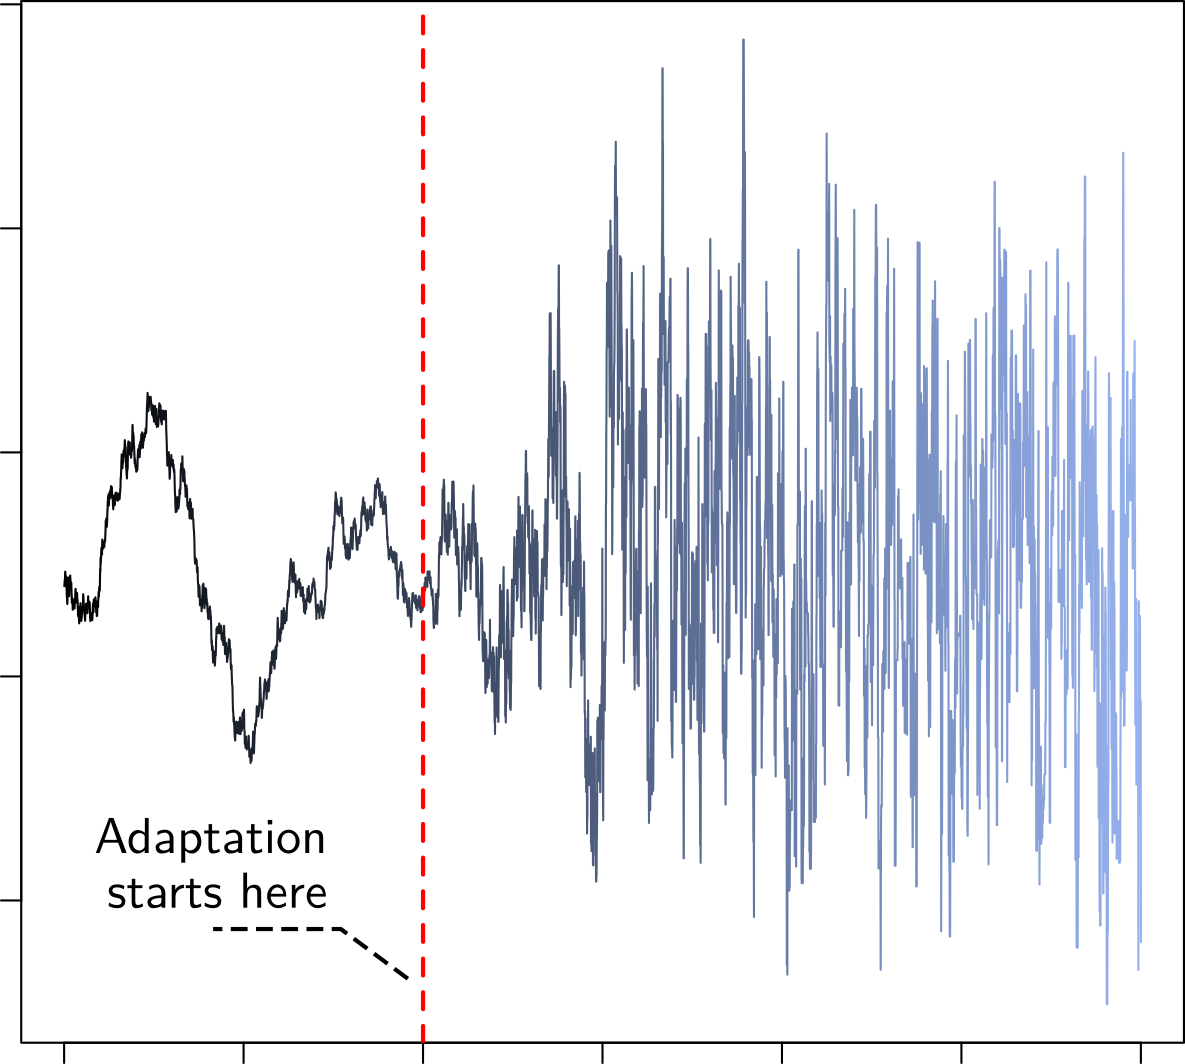
\includegraphics[width=.8\linewidth]{mcmc.png}\\Bayesian, Non-parametric, Spatial}}
	\uncover<3->{\byside{.32}{Computer Science}{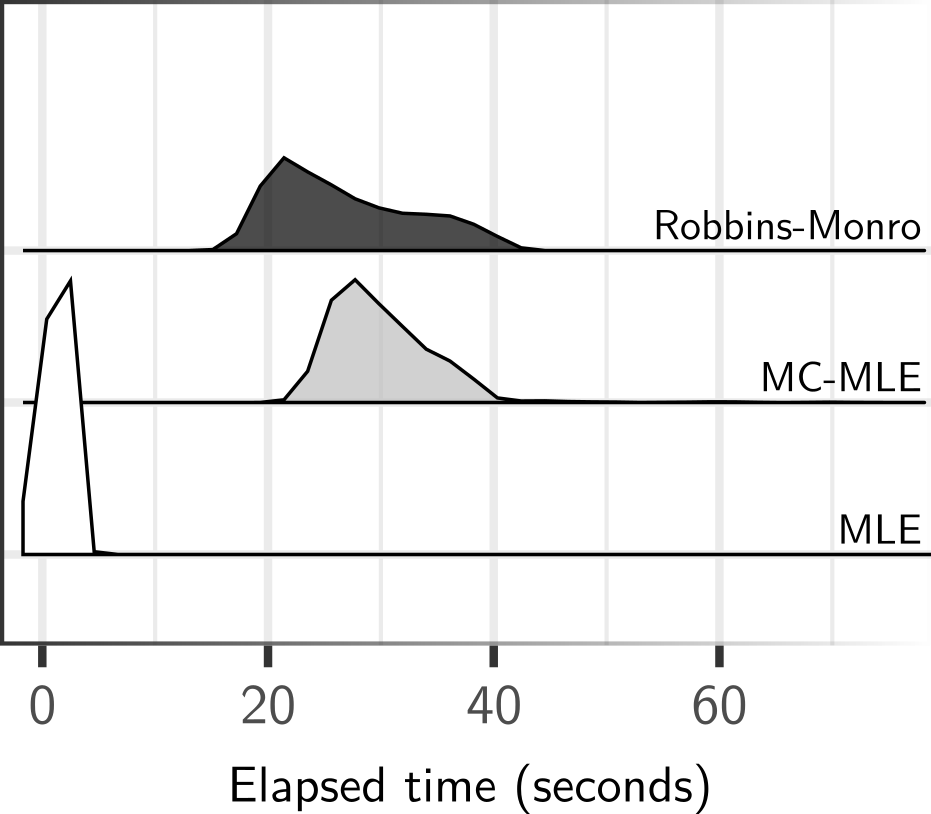
\includegraphics[width=.8\linewidth]{time.png}\\ parallel computing, HPC, software}}
	\uncover<4->{\byside{.32}{Complex Systems}{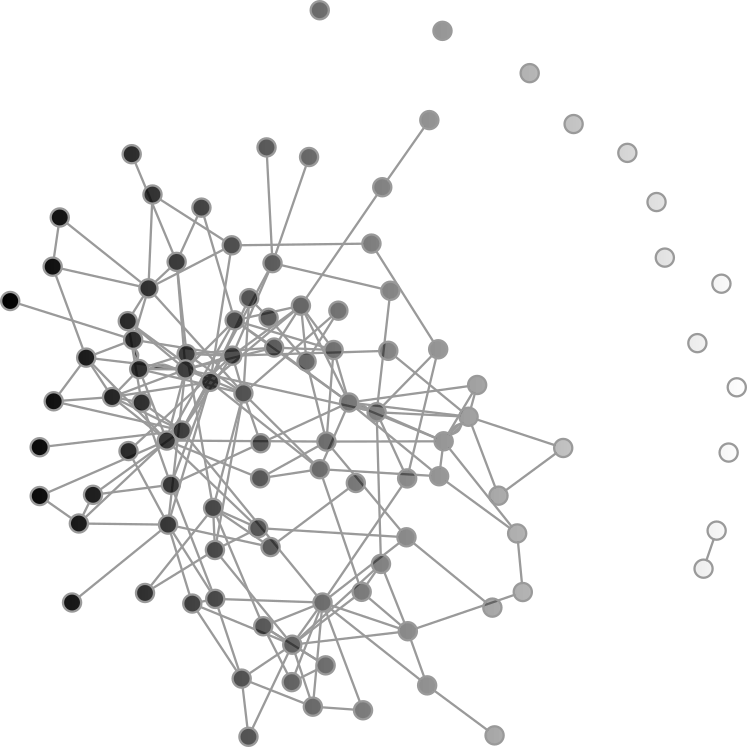
\includegraphics[width=.8\linewidth]{complex.png}\\social, biological, technical}}
	
	
\end{frame}

\frame{\frametitle{Contents}
	\tableofcontents
	\vfill
	You can download the slides from\large{} {\color{usccardinal}\url{https://github.com/gvegayon/faculty-talk}}\normalsize
}

%\begin{frame}
%		\Large Career path\bigskip\normalsize
%	\begin{center}
%		\begin{tabular}{*{3}{m{.25\linewidth}<\centering}}
%			Master Economics and Public Policy & %
%			Master in Social Science \linebreak  Economics &
%			PhD in Biostatistics \linebreak Statistical Computing 
%			\\
%			(UAI)  & (Caltech) & (USC)
%		\end{tabular}
%	\end{center}\bigskip
%\end{frame}



% ------------------------------------------------------------------------------
\section{Part 1: On the Prediction of Gene Functions Using Phylogenetic Trees}

\begin{frame}[t]
\usebeamertemplate{section intro}{}{}
\textcolor{uscgold}{
\Large {\bf Part 1: On the Prediction of Gene Functions Using Phylogenetic Trees} \vskip0.25em
\large \textit{Joint with}: Paul D Thomas, Paul Marjoram, Huaiyu Mi, Duncan Thomas, and John Morrison \\
(\small Accepted at \textit{PLOS Computational Biology})
}
\end{frame}


% ------------------------------------------------------------------------------

\begin{frame}[c]
%	\frametitle{Uncovering the role of genes}
	
	\Large Is gene \textit{XYZ} involved in process \textit{ABC}?\normalsize\bigskip
	
	\begin{minipage}[t]{.33\linewidth}
		\centering
		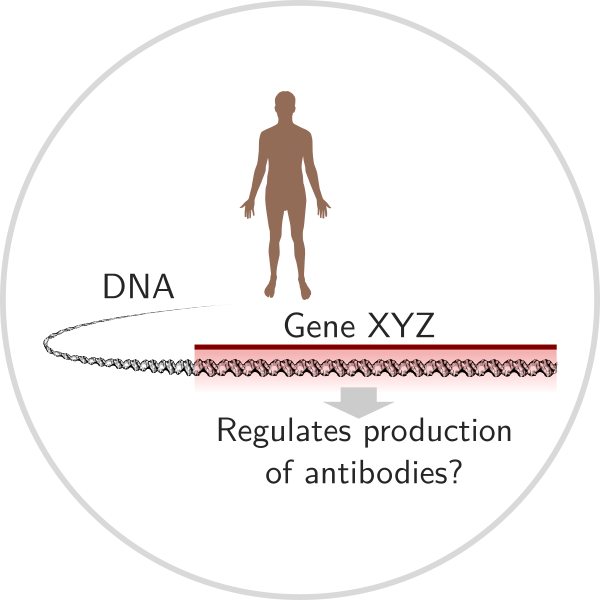
\includegraphics[width=1\linewidth]{aphylo-data-0.png} \\
		Complex to directly assess
	\end{minipage}\hfill
	\uncover<2->{\begin{minipage}[t]{.33\linewidth}
		\centering
		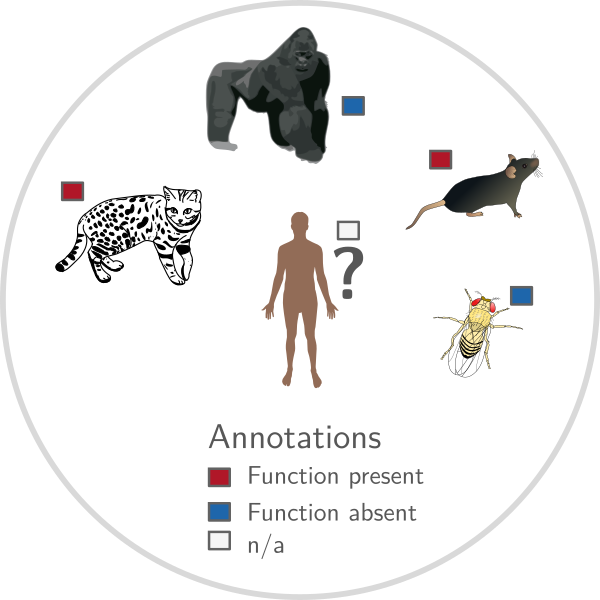
\includegraphics[width=1\linewidth]{aphylo-data-1.png}\\
		But we may know from other species
	\end{minipage}}\hfill
	\uncover<3->{\begin{minipage}[t]{.33\linewidth}
		\centering
		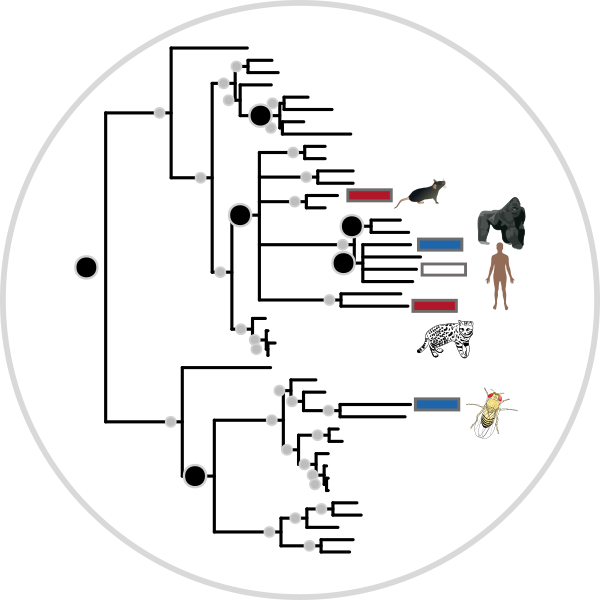
\includegraphics[width=1\linewidth]{aphylo-data-2.png}\\
		And we further know how these \textit{genetically} connected
	\end{minipage}}\hfill
	
\bigskip\uncover<4>{\raggedleft\Large ... let's rephrase the question. \normalsize}

\end{frame}

\begin{frame}[c,label=aphylo-prob-diagram]
	\begin{center}
		\normalsize Is the human gene \textbf{XYZ} involved in process \textbf{ABC}, \uline{given what we know about that for other \textit{related} species}?
	\end{center}
	
	\begin{figure}
		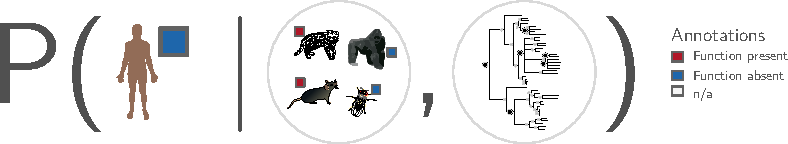
\includegraphics[width=.9\linewidth]{aphylo-data-probability.pdf}
	\end{figure}\pause
	\Large \bigskip\hfill... Where is all this data?\normalsize


\vfill\hfill\hyperlink{aphylographicalview}{\beamergotobutton{more}}

\end{frame}

\begin{frame}[c,label=geneontology]
	\frametitle{The Gene Ontology Project}
	\begin{minipage}[m]{.33\linewidth}
		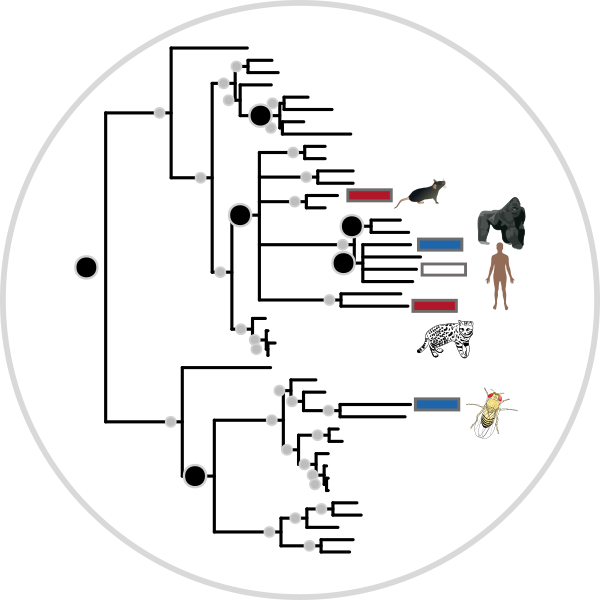
\includegraphics[width=1\linewidth]{aphylo-data-2.png}
	\end{minipage}\hfill
	\begin{minipage}[m]{.66\linewidth}
		\begin{figure}
		
\includegraphics[width=.5\linewidth]{go-logo.png}
		\end{figure}
	\begin{itemize}
		\item<2-> $\sim$ 15,000 phylogenetic trees		
		\item<3-> $\sim$ 8 million annotations
		\item<4-> $\sim$ 600 thousand on human genes
		\item<5-> $\sim$ $<$ 10\% are based on experimental evidence... \uncover<6->{Improving our knowledge on genetics is fundamental for advancing Biomedical Research}
	\end{itemize}
	\end{minipage}
\vfill \hfill
\Large \uncover<7->{Only on 2020, 2,000+ COVID-19 papers using the GO \href{https://scholar.google.com/scholar?as\_ylo=2020\&q="gene+ontology"+(covid+OR+coronavirus)}{(Google Scholar)}}\normalsize\\
\hfill\hyperlink{go-functions-types}{\beamergotobutton{more}}

\end{frame}

%--------------------------------------------------------------------------------
\newcommand{\oinclude}[2]{\only<#1>{\includegraphics[width=\tmpwdth,clip,trim={0 0 0 2cm}]{#2}}}


%%-------------------------------------------------------------------------------
%\begin{frame}
%	\frametitle{An evolutionary model of gene functions}
%	
%	Imagine a relay race...
%	\begin{figure}
%		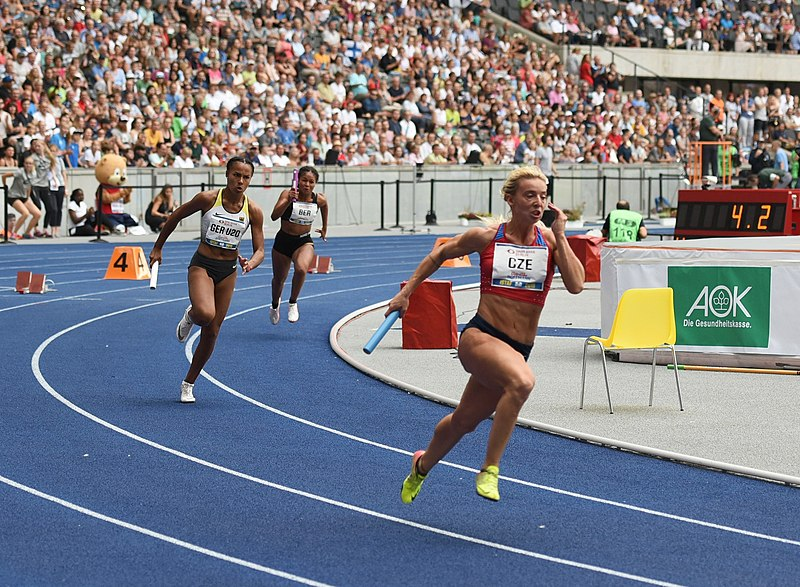
\includegraphics[width=.55\linewidth]{800px-2019-09-01_ISTAF_2019_4_x_100_m_relay_race_(Martin_Rulsch)_10.jpg}
%		\caption{ISTAF 2019 4 x 100 m relay race (Martin Rulsch, \href{https://commons.wikimedia.org/wiki/File:2019-09-01_ISTAF_2019_4_x_100_m_relay_race_(Martin_Rulsch)_10.jpg}{wikimedia})}
%	\end{figure}
%	
%\end{frame}

%--------------------------------------------------------------------------------
%\newcommand{\oinclude}[2]{\only<#1>{\includegraphics[width=\tmpwdth,clip,trim={0 0 0 2cm}]{#2}}}

\begin{frame}[t, label=aphylo-good]
	\frametitle{An evolutionary model of gene functions}
	
	\begin{minipage}[m]{.34\linewidth}
		\small
		%	The AUC for this analysis is 0.91 and the Mean Absolute Error is 0.34
		\uncover<1->{\textbf{Family: PTHR11258}}\\
		\uncover<1->{%
			\textbf{Type:} Molecular Function\\
			\textbf{Name:} 2'-5'-oligoadenylate synthetase activity\\
			\textbf{Desc:}  \href{http://amigo.geneontology.org/amigo/term/GO:0001730}{\alert{GO:0001730}} involved in the process of cellular antiviral activity (wiki on \href{https://en.wikipedia.org/wiki/Interferon}{\alert{interferon}}).
		}\\
		\uncover<2->{%
			\textbf{MAE:} 0.34 \\
			\textbf{AUC:} 0.91%
		}
	
		\uncover<3->{
			\Large This model is implemented in the \textbf{aphylo} R package
		}
	
		\vfill
		\hyperlink{aphylo-good-details}{\beamerbutton{see details}}
	\end{minipage}
	\begin{minipage}[m]{.65\linewidth}
		\centering
		
		\mode<beamer>{
			\only<1>{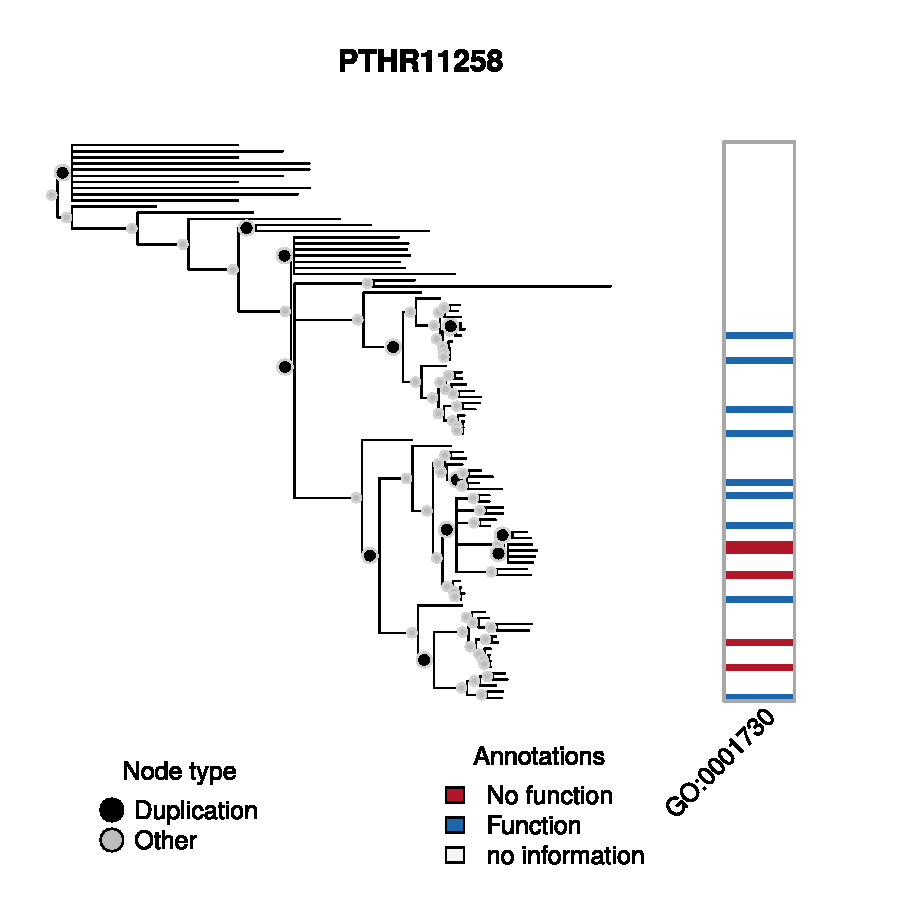
\includegraphics[width=.9\linewidth, clip, trim={0 0 0 2cm}]{example-trees-good1-parts-1.pdf}}%
			\only<2->{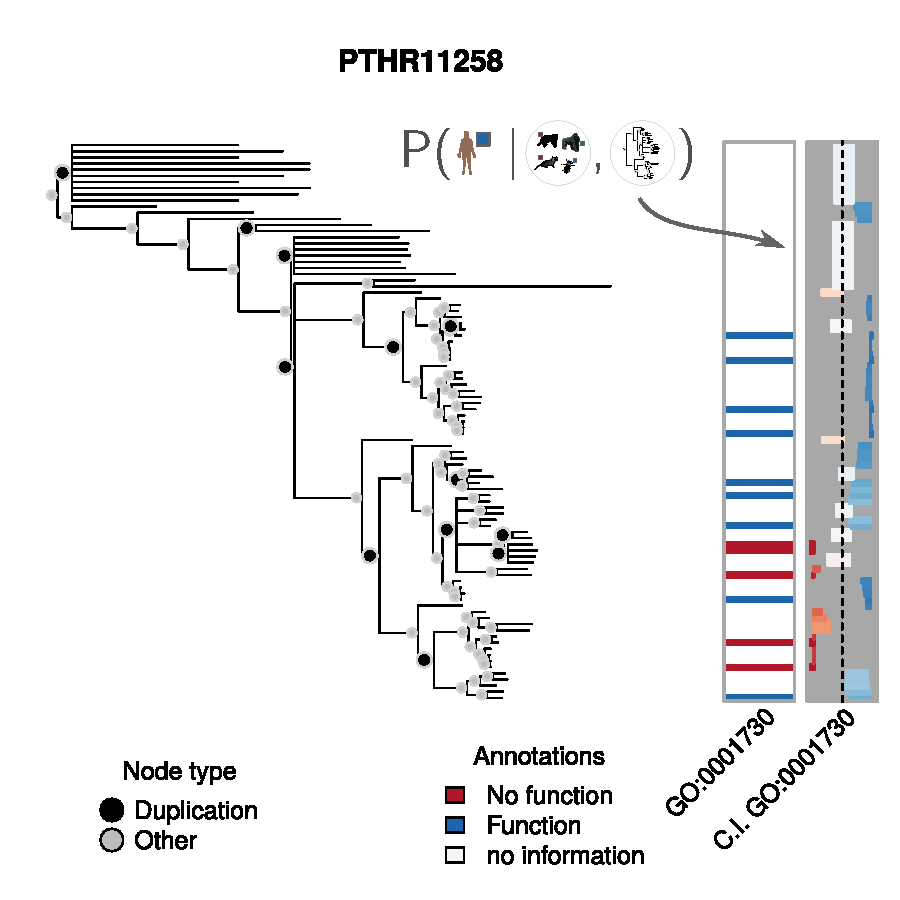
\includegraphics[width=.9\linewidth, clip, trim={0 0 0 2cm}]{example-trees-good1-parts-1b.pdf}}
		}
		\mode<handout>{
			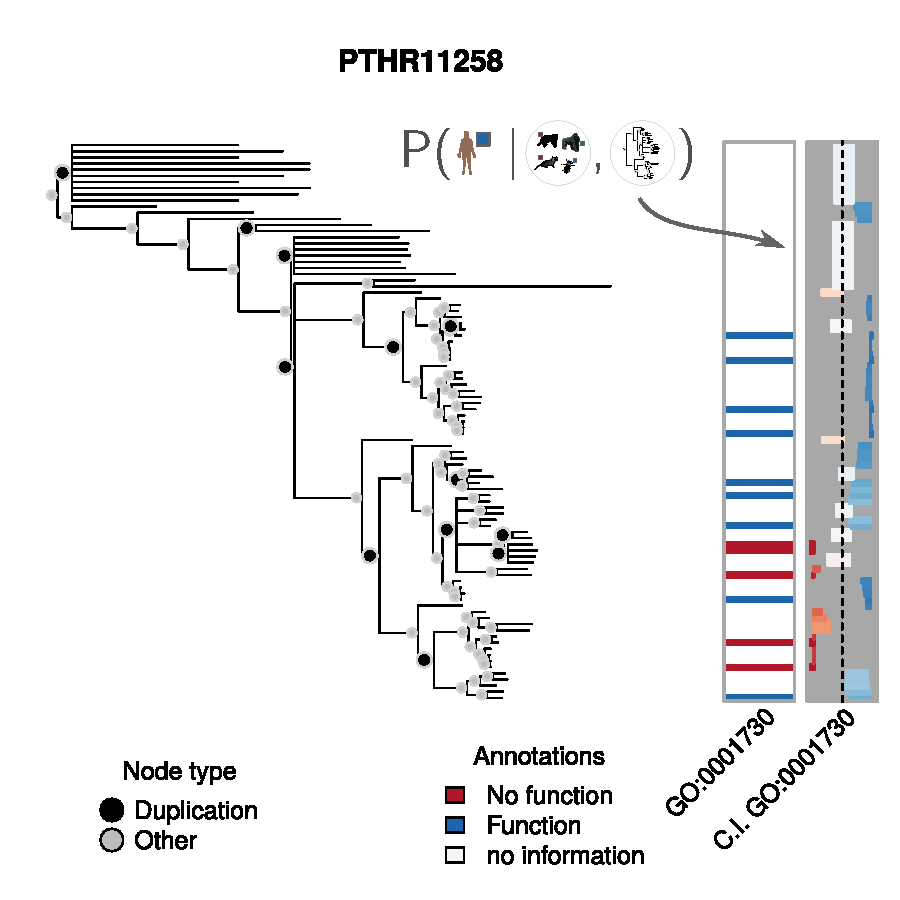
\includegraphics[width=.9\linewidth, clip, trim={0 0 0 2cm}]{example-trees-good1-parts-1b.pdf}
		}
	
		
	\end{minipage}
\end{frame}

%--------------------------------------------------------------------------------
\begin{frame}
	\frametitle{Computational features of \textbf{aphylo}}
	\begin{minipage}[m]{.55\linewidth}
		\vspace{-1cm}\raggedleft
\includegraphics[width=.35\linewidth]{aphylo-logo.png}\\\vspace{-.5cm}
		\raggedright
		\small
		\shadowbox{Baseline features}
		\begin{itemize}
			\item<2-> Parsimony: Independence across functions/siblings.
			\item<3-> Post-order Tree traversal: Linear complexity $O(|\mbox{tree}|)$.
		\end{itemize}
		\uncover<4->{\shadowbox{Additional features}}
		\begin{itemize}
			\item<5-> Reduced pruning sequence: Induced sub-tree of nodes connected to annotated leafs\\ $\implies$ Complexity $O(\left|\mbox{Induced sub-tree}\right|)\leq O(|\mbox{tree}|)$
			\item<6-> Implemented in C++ (\textbf{pruner} library)
		\end{itemize}
	\end{minipage}\hfill
	\begin{minipage}[m]{.44\linewidth}
		\centering
		\uncover<5->{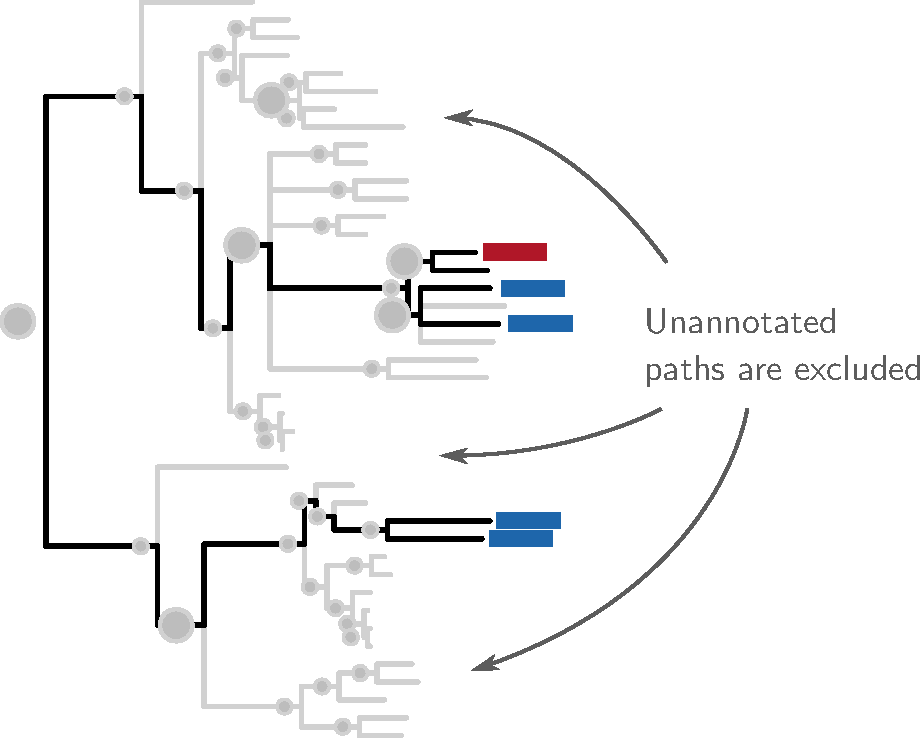
\includegraphics[width=1\linewidth]{reduced-sequence.pdf}}
	\end{minipage}
\end{frame}

\begin{frame}[c,label=aphylo-results-brief]
	\frametitle{Results: What does aphylo brings to the table?}
	\begin{center}
		
\includegraphics[width=.2\linewidth]{aphylo-logo.png}
	\end{center}
	
	\uncover<1->{\begin{minipage}[t]{.24\linewidth}\centering
		\shadowbox{Large scale}\\\small
		Estimate \textbf{pooled-data models} involving
		\textbf{hundreds of families}\\
		(1,300 genes at a time)
	\end{minipage}}\hfill
	\uncover<2->{\begin{minipage}[t]{.24\linewidth}\centering
		\shadowbox{Interpretable}\\\small
		Pooled-data model provides inference
		\textbf{aligned with theoretical results}\\
		(gene duplication is key)
	\end{minipage}}\hfill
	\uncover<3->{\begin{minipage}[t]{.24\linewidth}\centering
		\shadowbox{Fast}\\\small
		Computational efficiency
		allows making \textbf{inference and prediction fast}\\
		(1 second vs 2 hours)
	\end{minipage}}\hfill
	\uncover<4->{\begin{minipage}[t]{.24\linewidth}\centering
		\shadowbox{Accuracy}\\\small
		Outperforms state-of-the-art
		phylo-models\\
		(0.72 vs 0.60 AUC)
	\end{minipage}}
\vfill\hfill\hyperlink{aphylo-results-overview}{\beamergotobutton{details}}
\end{frame}




%% ------------------------------------------------------------------------------
%\begin{frame}
%	\frametitle{Predicting Gene Functions}
%	
%	\begin{center}
%		
\includegraphics[width=3cm]{aphylo-logo.png}
%	\end{center}\vspace{-1.5cm}
%	
%	\Large I built a model that is\normalsize
%	
%	\uncover<2->{\byside{.32}{Scalable}{Prediction on thousands of genes within seconds}\hfill}
%	\uncover<3->{\byside{.32}{Biologically accurate}{Inference on pooled-data is plausible and results match intuition}\hfill}
%	\uncover<4->{\byside{.32}{Competitive}{Beats state-of-the-art phylo-based models}}
%	
%	\bigskip
%	
%	\raggedleft \Large \uncover<5->{... a contribution to biomedical research.}\normalsize
%	
%\end{frame}


% ------------------------------------------------------------------------------
\section{Part 2: Exponential Random Graph Models for Small Networks}
% \frame{\frametitle{Contents}\tableofcontents}

\begin{frame}[t]
\usebeamertemplate{section intro}{}{}
\textcolor{uscgold}{
\Large {\bf Part 2: Exponential Random Graph Models for Small Networks} \vskip0.25em
\large \textit{Joint with}: Andrew Slaughter and Kayla de la Haye \\
({\small published in the journal \textit{Social Networks}})
}
\end{frame}

%-------------------------------------------------------------------------------
\begin{frame}[c]
\frametitle{Social Networks}

\begin{minipage}[m]{.3\linewidth}
	\begin{itemize}
		\item<2-> If COVID-19 has taught us something it is that networks matter.
		\item<3-> And especially small networks: Families, teams, friends, etc. \uncover<4->{The cornerstone of larger social systems.}
		\item<5-> We can study networks using ERGMs.
	\end{itemize}
\vfill
\uncover<1->{\tiny \textbf{Data:} Friendship network of a UK university faculty from \textbf{igraphdata}. \textbf{Viz:} R package \textbf{netplot} (yours truly, \href{https://github.com/usccana/netplot}{github.com/usccana/netplot})\normalsize}
\end{minipage}\hfill
\begin{minipage}[m]{.69\linewidth}
\begin{figure}
	\centering
	\includegraphics<1->[height=.85\textheight]{ukfaculty-igraph.pdf}
\end{figure}

\end{minipage}


\end{frame}

%-------------------------------------------------------------------------------
\begin{frame}
\frametitle{What are Exponential Random Graph Models}

Exponential Family Random Graph Models, aka \alert{ERGMs} are:\pause

\begin{itemize}
\item Statistical models of (social) networks.\pause
\item Not about individual ties, but about local structures (sufficient statistics).\pause
\begin{figure}
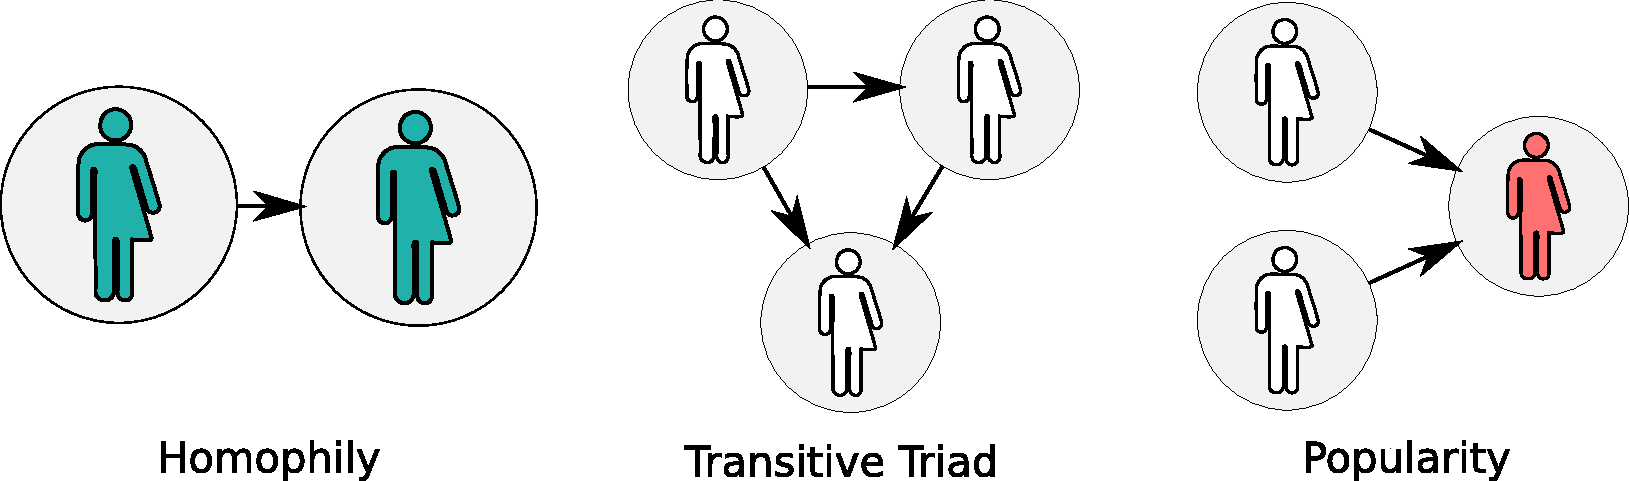
\includegraphics[width=.6\linewidth]{friendly-terms.pdf}
\end{figure}
%\item Used to test hypotheses 
\end{itemize}

\end{frame}

\begin{frame}[t,label=discrete-exponential]
	
	\frametitle{Discrete Exponential-Family Models}
	
	\begin{figure}
		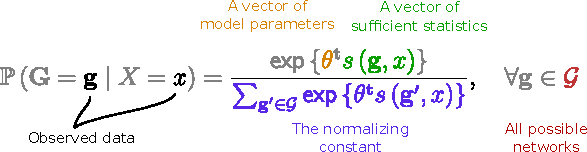
\includegraphics[width=.7\linewidth]{parts-of-ergm.pdf}
	\end{figure}\pause
	
	\vfill
		
	\begin{itemize}
		%\item<2-> Focused on sufficient statistics $\s{\graph,x}$ \uncover<3->{\textbf{e.g.}\\Two Bernoulli, a.k.a. Erd\H{o}s-R\'enyi, random graphs}.
		\item For any directed graph of size $n$, there are $2^{n(n - 1)}$ possible realizations.\pause
		\item A directed graph of size 5 has 1,048,576 possible configurations!\pause
		\item Most (all) applications use \textbf{approximations}...\pause{} yet, for sufficiently small graphs we ``can be exact.''
	\end{itemize}\pause

	\Large ... I implemented ``exact calculations'' in the \textbf{ergmito} package (ERGM\textit{ito})\normalsize
	
	\vfill\hfill\hyperlink{discrete-exponential-theory}{\beamergotobutton{more theory}} %
	\hyperlink{ergm-terms}{\beamergotobutton{more terms}}

	
\end{frame}

\begin{frame}
	\frametitle{Computational Complexity: ergmito}
	\begin{minipage}[m]{.4\linewidth}
		\shadowbox{Premise}
		\begin{itemize}
			\item<2-> Full enumeration $\neq$ All networks with $k$ ties
		\end{itemize}
		\uncover<3->{\shadowbox{Extra features}}
		\begin{itemize}
			\item<4-> \textit{Iso-support} structures (model) recycled
			\item<5-> Core algorithm written in C++
			\item<6-> Parallel computing using \textbf{OpenMP}
		\end{itemize}
	\end{minipage}\hfill
	\begin{minipage}[m]{.59\linewidth}
		\centering
		\uncover<4->{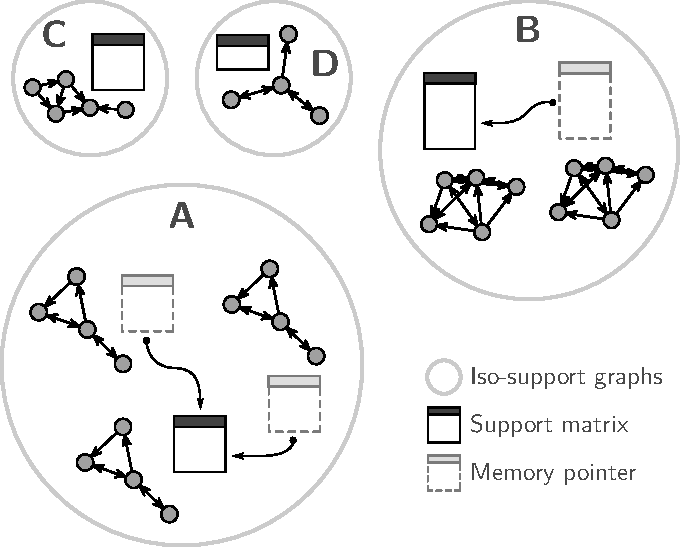
\includegraphics[width=1\linewidth]{ergm-computing.pdf}}
	\end{minipage}
	\uncover<8->{Simple ERGMito with 80,000 nodes $\sim$ 4s}
\end{frame}


% % ------------------------------------------------------------------------------
% \begin{frame}
% \frametitle{ERGMs for Small Networks}
% 
% From the methodological point of view, current methods are great, but:\pause
% 
% \begin{itemize}
% \item Possible accuracy issues (error rates)\pause
% \item Prone to degeneracy problems (sampling and existence of MLE)\pause
% \item It is not MLE...
% \end{itemize}
% 
% \end{frame}


\begin{frame}[c]
	\usebeamertemplate{section intro}{}{}
	\textcolor{uscgold}{
		\Large \textbf{ergmito}: Featured Example
	}
\end{frame}


%-------------------------------------------------------------------------------
\begin{frame}[t, label=ergmito-applied]
	\centering
	\mode<beamer>{
		\includegraphics<1-2>[width=.95\linewidth]{fig/ci-ergm-all-nets-wide.pdf}%
		\includegraphics<3>[width=.95\linewidth]{fig/ci-ergm-all-nets-wide-edges.pdf}%
		\includegraphics<4>[width=.95\linewidth]{fig/ci-ergm-all-nets-wide-transitivity.pdf}%
		\includegraphics<5>[width=.95\linewidth]{fig/ci-ergm-all-nets-wide.pdf}%
		\includegraphics<6>[width=.95\linewidth]{fig/ci-ergm-all-nets-wide-sender.pdf}%
		\includegraphics<7->[width=.95\linewidth]{fig/ci-ergm-all-nets-wide-all.pdf}
	}%
	\mode<handout>{
		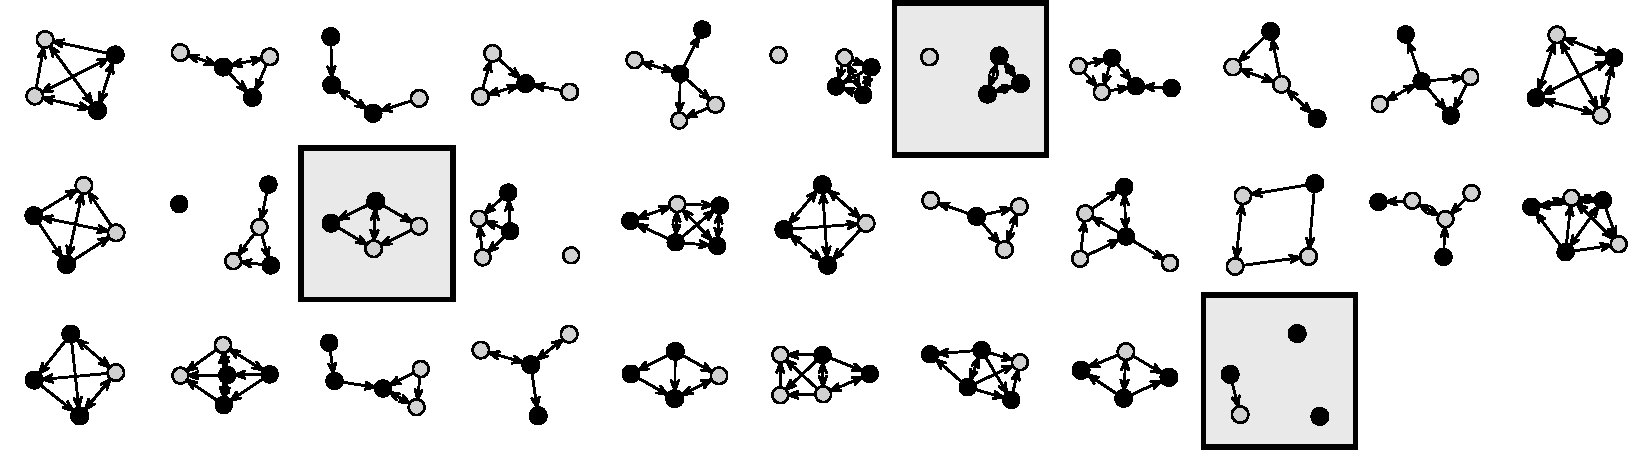
\includegraphics[width=.95\linewidth]{fig/ci-ergm-all-nets-wide-all.pdf}
	}

	\vspace{-.75cm}\hfill\hyperlink{ergmito-teams-data}{\beamergotobutton{experiment}} \\ \vspace{.75cm}

	\small\pause
	\begin{minipage}[t]{.38\linewidth}
	\begin{center}
		\shadowbox{Key findings}\pause
	\end{center}
	\begin{itemize}
		\item Low density.\pause
		\item High balance (transitive triads).\pause
		\item No evidence of gender homophily.\pause
		\item Females are more likely to ask for advice.\pause
	\end{itemize}
	\end{minipage}\hfill
	\begin{minipage}[t]{.58\linewidth}
	\begin{center}
	\shadowbox{What's different \tiny(from regular ERGMs)\normalsize?}
	\end{center}\pause
		
	\begin{itemize}
		\item Interaction effects: $\text{edges} \times \isone{n = 5}$.\pause
		\item Constrained support: $\text{edge} > 4$.\pause
		\item Transformed variables: $(\text{Homophily})^{1/2}$.\pause
		\item Bootstrapping: 1,000 replicates in less than 1.5 minutes...\pause \\
		... if you are lucky, using ``regular'' ERGMs would take you about 5 hours.
	\end{itemize}
	\end{minipage}\hfill
	\vfill\hfill%
	\only<1->{%
		\hyperlink{ergmito-table}{\beamergotobutton{details}} %
		\hyperlink{ergmito-gof}{\beamergotobutton{gof}} %
		\hyperlink{example-data-ergm}{\beamergotobutton{data}}%
	}
\end{frame}


\begin{frame}[c,label=ergmito-results-brief]
	\frametitle{Results: What does \textbf{ergmito} brings to the table?}
	\begin{center}
		
\includegraphics[width=.2\linewidth]{ergmito-logo.png}
	\end{center}
	
	\uncover<1->{\begin{minipage}[t]{.24\linewidth}\centering
			\shadowbox{Theoretical Goodies}\\\small
			Higher convergence race, lower bias, lower type-I error, higher power, ...
	\end{minipage}}\hfill
	\uncover<2->{\begin{minipage}[t]{.24\linewidth}\centering
			\shadowbox{Fast}\\\small
			Orders of magnitude faster than other methods\\
			(x200 faster in some cases)
	\end{minipage}}\hfill
	\uncover<3->{\begin{minipage}[t]{.24\linewidth}\centering
			\shadowbox{Flexible}\\\small
			Arbitrary transformations and constrains\\
			(interaction effects, for example)
	\end{minipage}}\hfill
	\uncover<4->{\begin{minipage}[t]{.24\linewidth}\centering
			\shadowbox{The right tool}\\\small
			For ego networks, families, small teams, etc.\\
			(
\includegraphics[width=2cm]{cran-downloads-ergmito.pdf} others think so)
	\end{minipage}}
\vfill\hfill\hyperlink{ergmito-simulations}{\beamergotobutton{more}}
\end{frame}



% ------------------------------------------------------------------------------
% ------------------------------------------------------------------------------
% ------------------------------------------------------------------------------
% ------------------------------------------------------------------------------
\section{Part 3: Current and Future Research}

%-------------------------------------------------------------------------------
\begin{frame}[t]
	\usebeamertemplate{section intro}{}{}
	\textcolor{uscgold}{
		\Large {\bf Part 3: Current and Future Research}
	}
\end{frame}

\begin{frame}[t,label=current-research]
\frametitle{Current Research}

\uncover<2->{\byside{.33}{Biology}{Extension of gene functional-evolution model using the ERGMs framework%
%\hyperlink{aphylo-current}{\beamergotobutton{more}}
}}\hfill
\uncover<3->{\byside{.33}{Criminology}{The role of social networks on police use of force}}\hfill
\uncover<4->{\byside{.33}{Sociology}{Using ERGMitos to model political discussion networks in Romania}}

\uncover<2->{\begin{minipage}[m]{.33\linewidth}
	\centering
	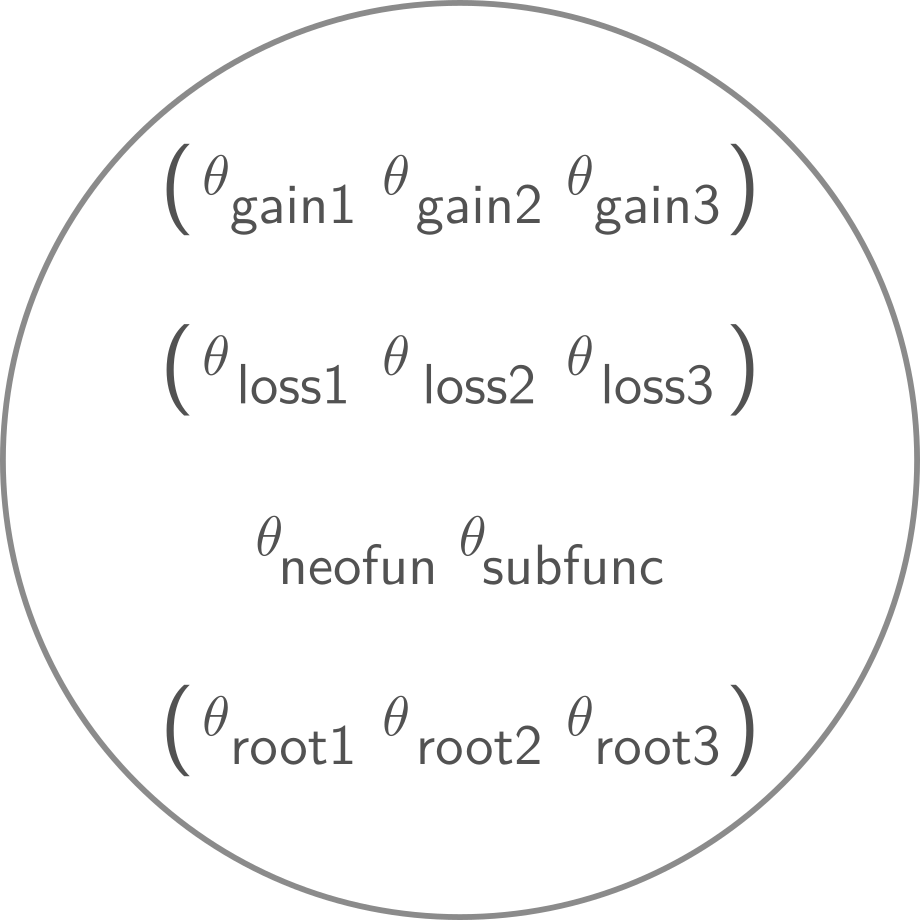
\includegraphics[width=.6\linewidth]{aphylo-ergm-eq2.png}
\end{minipage}}\hfill
\uncover<3->{\begin{minipage}[m]{.33\linewidth}
	\centering
	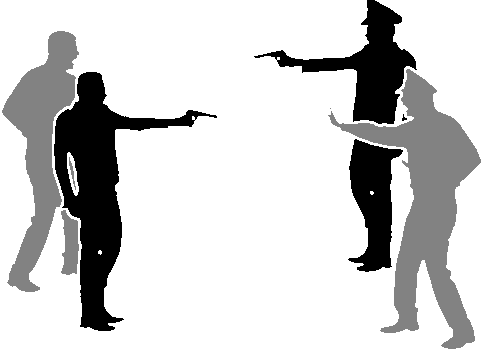
\includegraphics[width=.9\linewidth]{pointing.pdf}
\end{minipage}}\hfill
\uncover<4->{\begin{minipage}[m]{.33\linewidth}
	\centering
	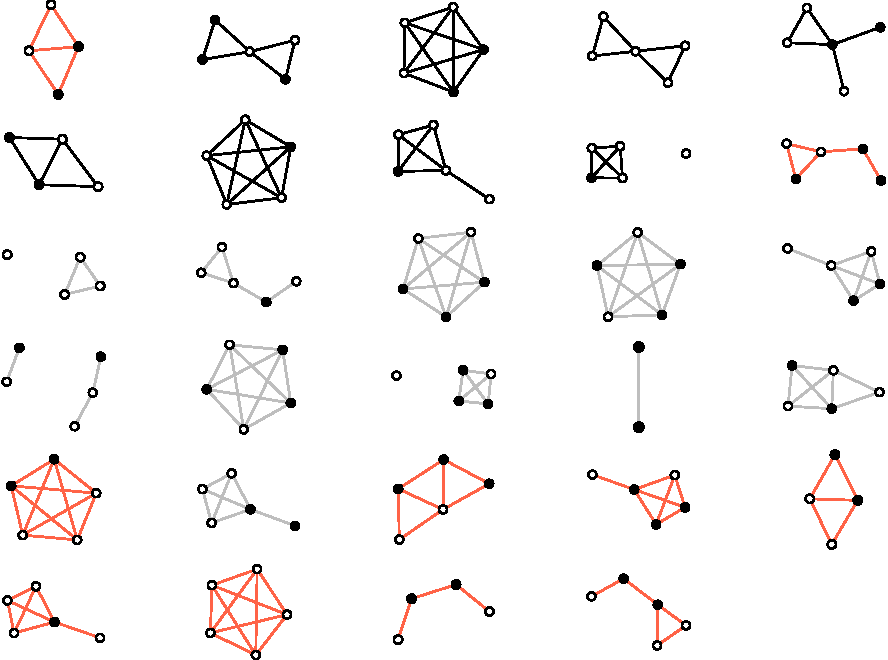
\includegraphics[width=.7\linewidth]{ergmitos-rumania.pdf}
\end{minipage}}

\end{frame}

\begin{frame}
	\frametitle{The future}
	\Large Continue developing scientific software... \normalsize
	\begin{figure}
		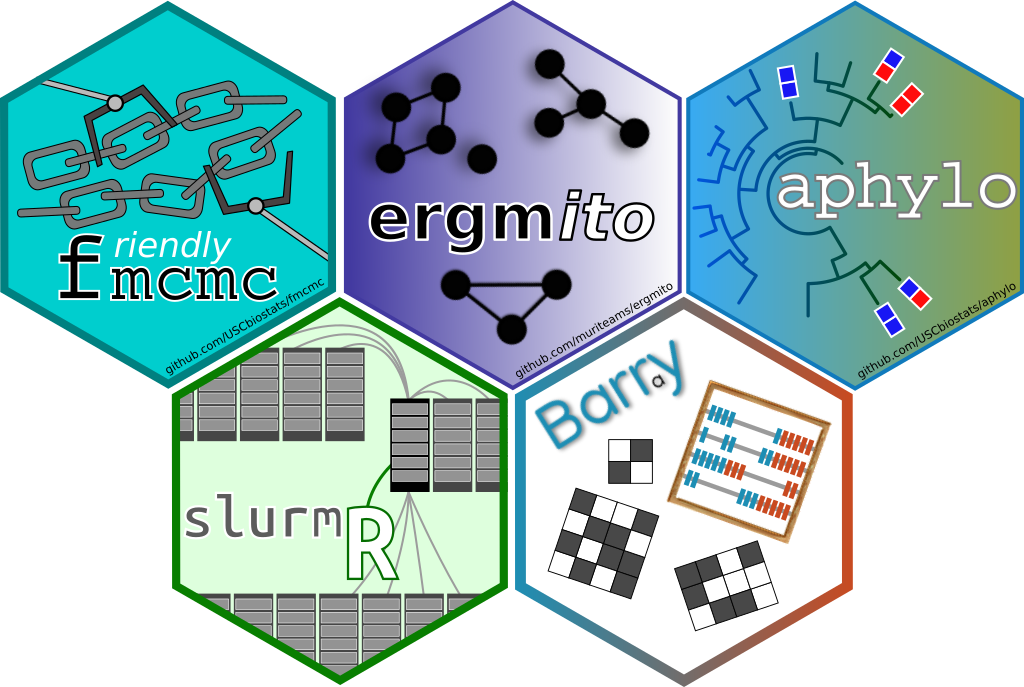
\includegraphics[width=.65\linewidth]{fig-packages/hexlogos.png}
	\end{figure}
\end{frame}

\begin{frame}
	\frametitle{The future: Keep building bridges}
	
	\mode<beamer>{
		\begin{figure}
					\centering
	\includegraphics<1>[width=.6\linewidth]{coauthors0.png}%
	\includegraphics<2->[width=.6\linewidth]{coauthors.png}
	\end{figure}
}
\mode<handout>{
	\begin{figure}
		\centering
	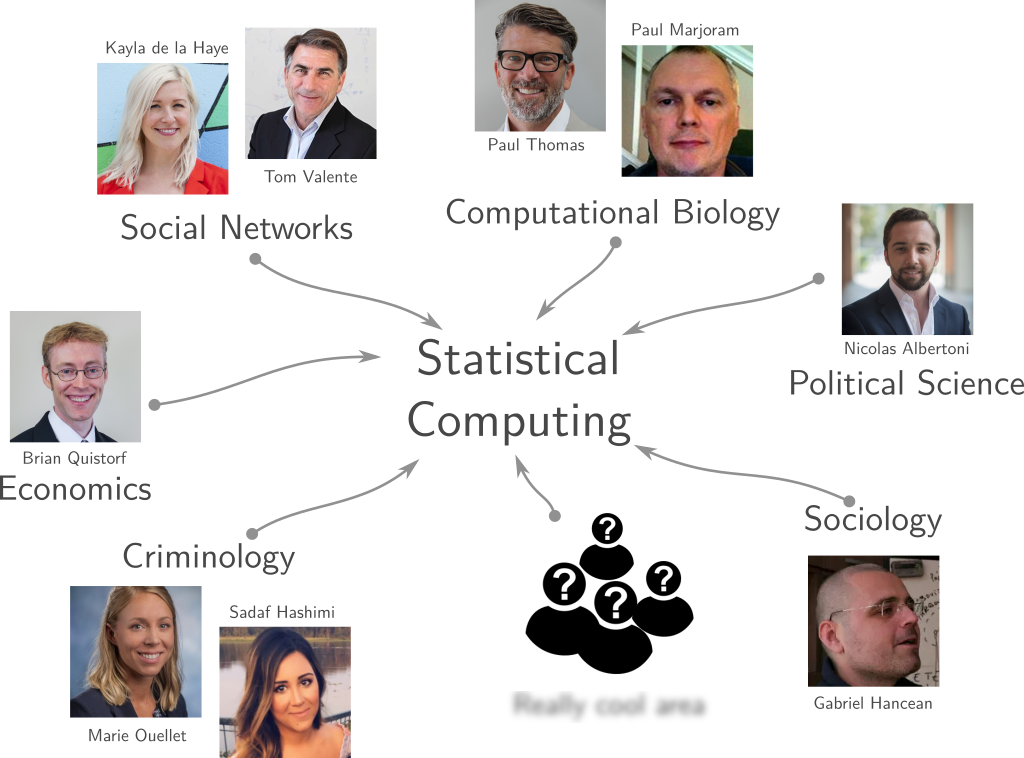
\includegraphics[width=.6\linewidth]{coauthors.png}
	\end{figure}
}
\hfill \uncover<2->{...you could be next!}\normalsize
\end{frame}

%%-------------------------------------------------------------------------------
%\begin{frame}[c]
%	\centering
%	\mode<beamer>{\scalebox{1.5}{
%			\only<1>{barray}\only<2->{\Huge{}{\color{usccardinal}Barr}\small{}a\Huge{}{\color{usccardinal}y}\normalsize}:
%	}}\mode<handout>{\Huge{}{\color{usccardinal}Barr}\small{}a\Huge{}{\color{usccardinal}y}\normalsize}
%	
%	\scalebox{1.5}{C++ header-only library for counting structures in binary arrays}
%	\pause
%	\vfill\raggedright {\footnotesize \href{https://en.wikipedia.org/wiki/The_Sniffing_Accountant}{``The Sniffing Accountant'' (Seinfeld, Season 5, Episode 4)}}
%\end{frame}

% ------------------------------------------------------------------------------
%\newcommand{\ultima}[3]{\begin{minipage}[t]{#1\linewidth}%
%		\begin{center}\shadowbox{#2}\end{center}\vspace{-.55cm}\hfill%	
%
%		\small#3\normalsize\end{minipage}%
%	}
%\begin{frame}[t]
%\frametitle{Concluding Remarks}
%\small
%\pause
%\color<4->{gray}
%\ultima{.3}{Before my dissertation}{%
%	\textbf{Predicting gene functions}
%	\begin{itemize}
%		\item ``Small scale''.
%		\item Detached from theory.
%	\end{itemize}\pause
%	
%	\textbf{ERGMs}
%	\begin{itemize}
%		\item Only approximations.
%		\item Small networks overlooked.
%		\item Limited alternatives for small nets.
%	\end{itemize}\pause
%}\color<4->{black}\hfill
%\ultima{.3}{After my dissertation}{%
%	\textbf{Predicting gene functions}
%	\begin{itemize}
%		\item Scale-up the problem.
%		\item More biology (via ERGMs).
%		\item New ways to look at phylo data.
%	\end{itemize}\pause
%
%	\textbf{ERGMs}
%	\begin{itemize}
%		\item Revisited exact methods.
%		\item New light on small networks.
%		\item Many opportunities for methodological innovations.
%	\end{itemize}\pause
%
%	\vfill
%	
%
%}\hfill
%\ultima{.39}{Products}{
%\textbf{Publications}
%
%6 journal publications (\tiny Journal of Open Source Software, Stata Journal, Journal of health and social behavior, Translational behavioral medicine, Social Science \& Medicine\small)\pause\textbf{+2 submitted} (\tiny PLOS Comp. Bio, Social Networks\small)\pause
%
%\textbf{Published software}
%\begin{itemize}
%\item ergmito 
\includegraphics[width=.3\linewidth]{cran-downloads-ergmito.pdf}
%\item slurmR 
\includegraphics[width=.3\linewidth]{cran-downloads-slurmr.pdf}
%\item fmcmc 
\includegraphics[width=.3\linewidth]{cran-downloads-fmcmc.pdf}
%\item netdiffuseR 
\includegraphics[width=.3\linewidth]{cran-downloads-netdiffuser.pdf}
%\end{itemize}\pause
%
%\textbf{Other tools}\\
%similR, gnet, aphylo, polygons, pruner, netplot, rphyloxml, jsPhyloSVG,\pause{} and {\large\color{usccardinal}\textbf{Barry}}
%
%}
%
%\end{frame}

% ------------------------------------------------------------------------------
\begin{frame}[c]
	\centering
	\usebeamertemplate{section intro}{}{}
	\textbf{%
		\color{uscgold}
		\Large Statistical and Computational Methods for Complex Systems\large %
	}

	\textbf{
		\color{uscgold}
		George G Vega Yon \\
		\url{https://ggvy.cl} \\
		vegayon@usc.edu
	}
	
	
\includemedia[%
	width=.3\linewidth,%
	height=.3\linewidth,%
	addresource=fig/walking-dead.mp4,%
	transparent,
	%transparent player background
	activate=pageopen,
	passcontext,
	%show VPlayer's right-click menu
	flashvars={
		source=fig/walking-dead.mp4
		&loop=true
		% loop video
	}
]{}{VPlayer.swf}
	
	
	\begin{center}
	\scalebox{2}{\textcolor{uscgold}{Thank you!}} 
	\end{center}
\end{frame}


\renewcommand{\section}[2]{}%
\appendix

% ------------------------------------------------------------------------------
% ------------------------------------------------------------------------------
% ------------------------------------------------------------------------------
% ------------------------------------------------------------------------------
% ------------------------------------------------------------------------------

% ------------------------------------------------------------------------------
\changemode{handout}

% ------------------------------------------------------------------------------
\begin{frame}[label=aphylographicalview,c]
	\frametitle{An evolutionary model of gene functions}
	\def\shadowsize{2pt}
	\definecolor{rootnode}{RGB}{0,159,211}
	\definecolor{innernode}{RGB}{90,159,89}
	\definecolor{leafnode}{RGB}{255,107,0}
	
	\begin{minipage}[m]{.60\linewidth}
		\begin{figure}
			\footnotesize
			\centering
			\mode<beamer>{
				\only<1>{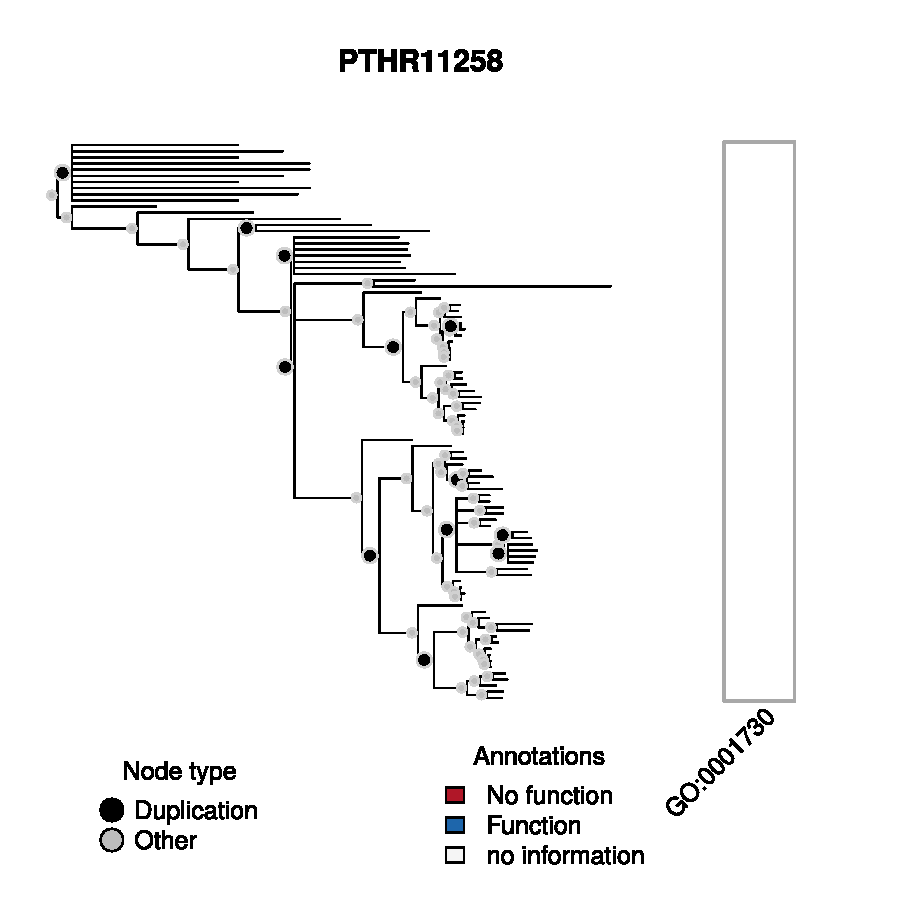
\includegraphics[width=.9\linewidth]{phylo-model2-0.pdf}}%
				\only<2>{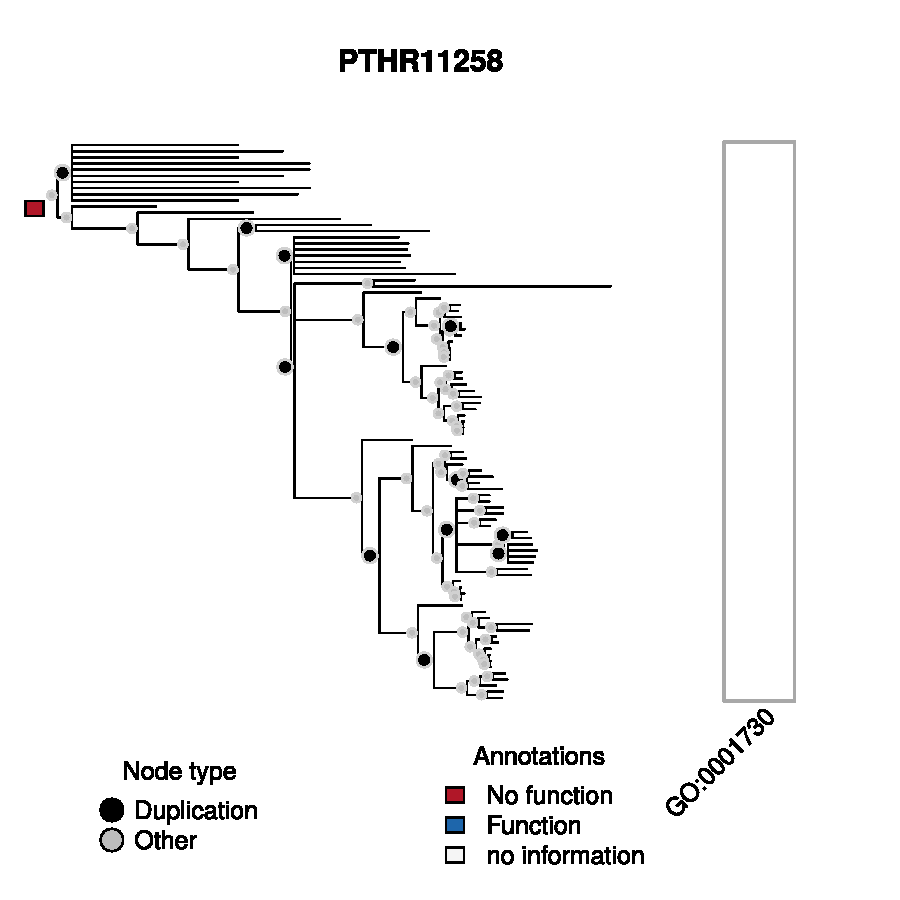
\includegraphics[width=.9\linewidth]{phylo-model2-1.pdf}}%
				\only<3>{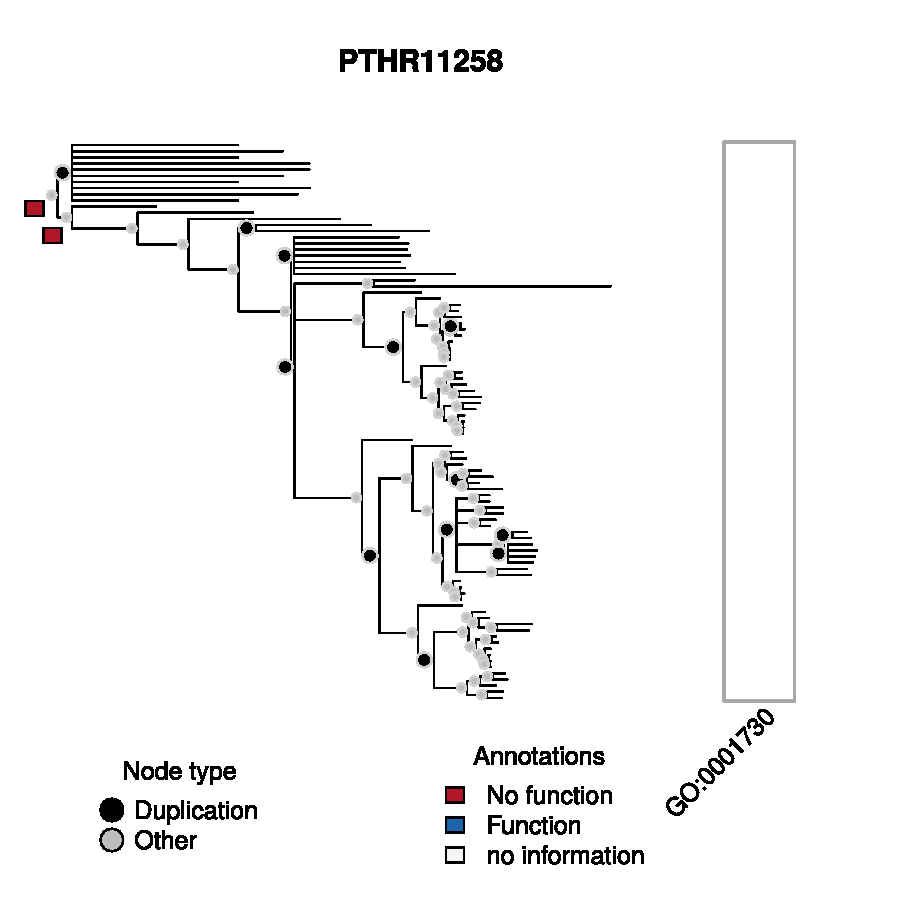
\includegraphics[width=.9\linewidth]{phylo-model2-2.pdf}}%
				\only<4>{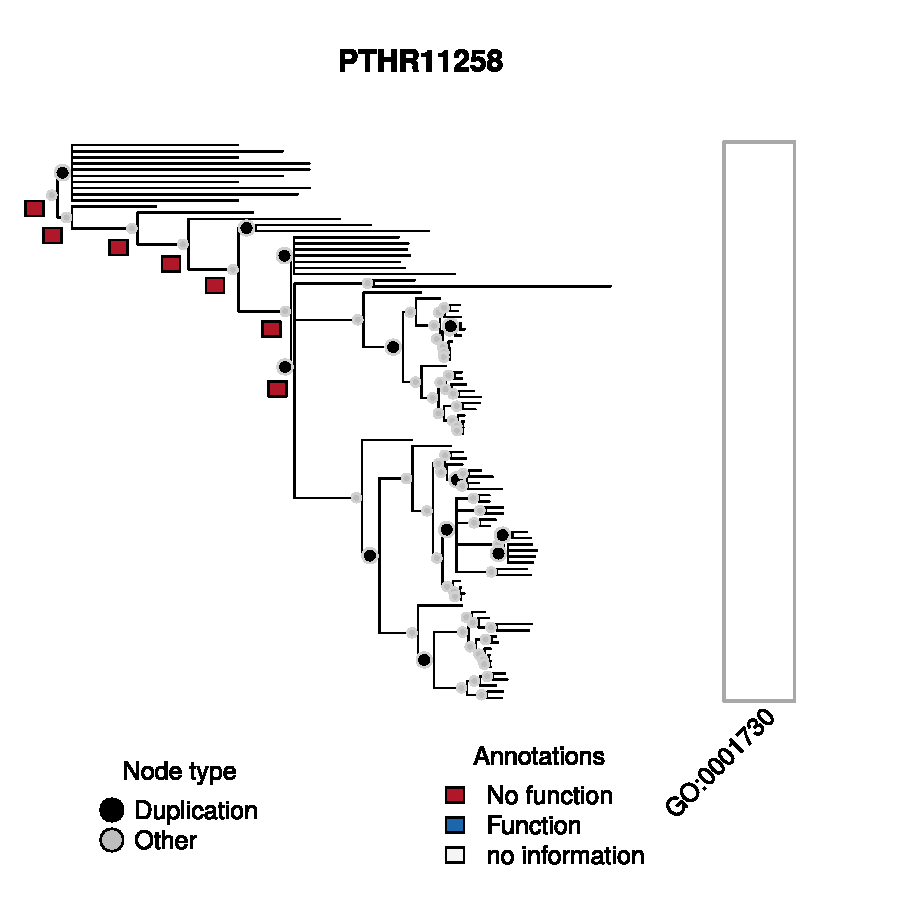
\includegraphics[width=.9\linewidth]{phylo-model2-3.pdf}}%
				\only<5>{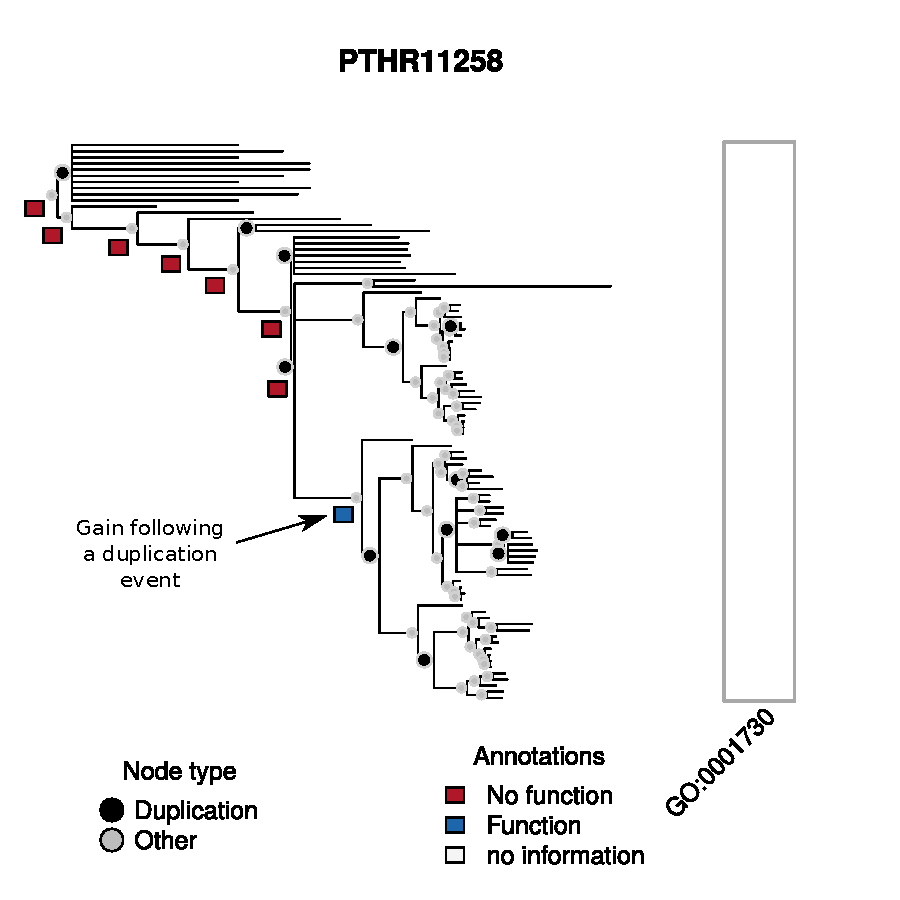
\includegraphics[width=.9\linewidth]{phylo-model2-4.pdf}}%
				\only<6>{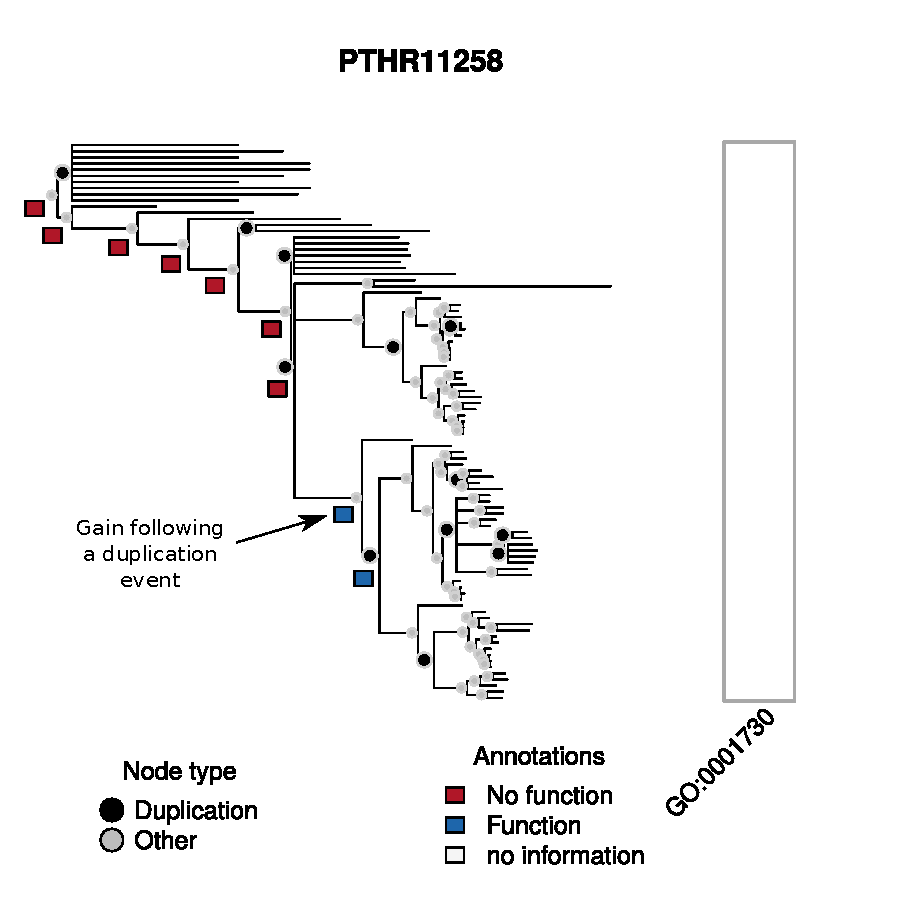
\includegraphics[width=.9\linewidth]{phylo-model2-5.pdf}}%
				\only<7>{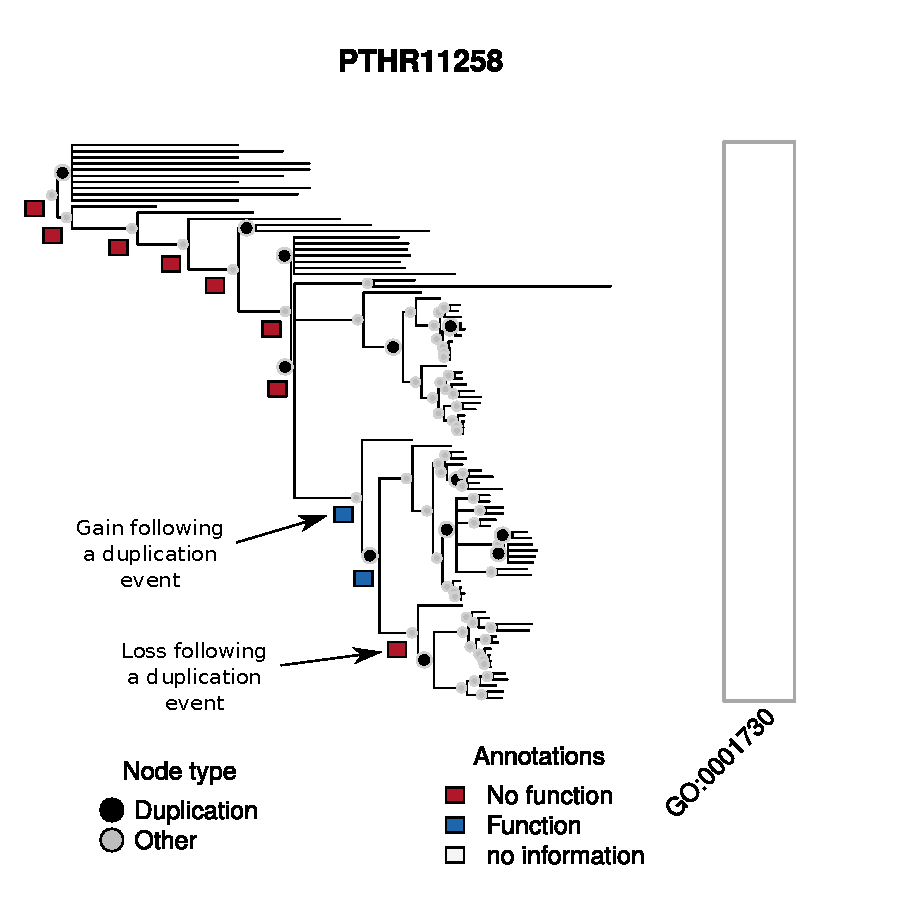
\includegraphics[width=.9\linewidth]{phylo-model2-6.pdf}}%
				\only<8>{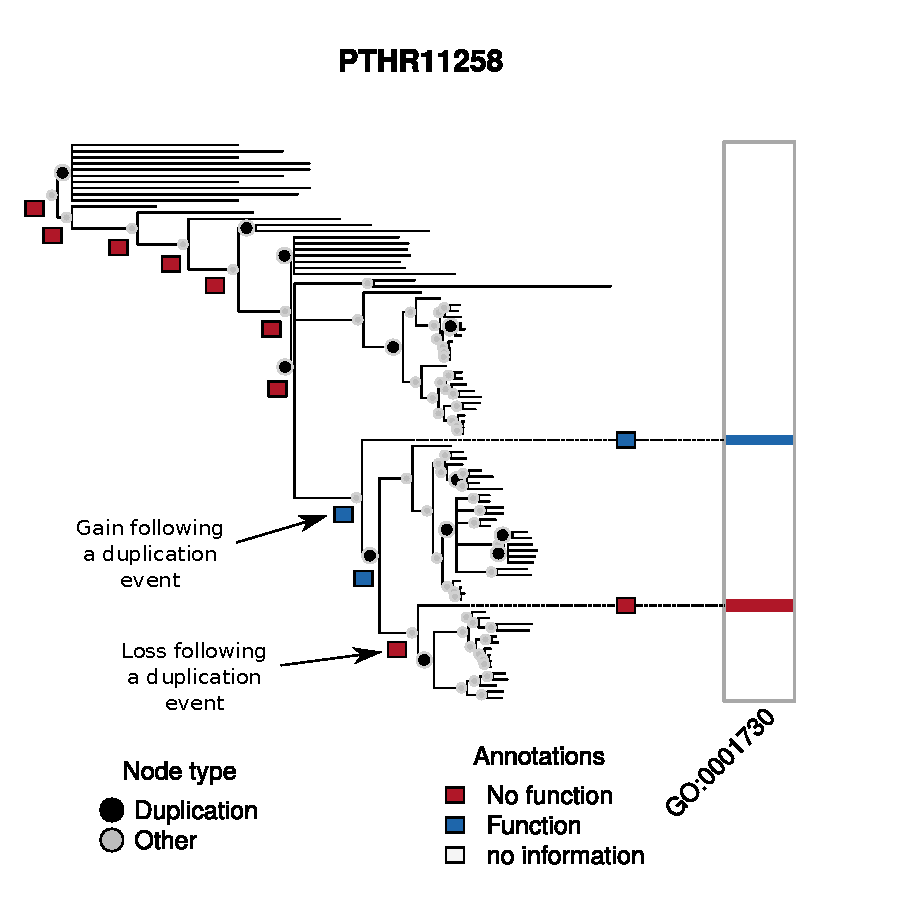
\includegraphics[width=.9\linewidth]{phylo-model2-7.pdf}}%
				\only<9->{\includegraphics[width=.9\linewidth]{phylo-model2.pdf}}%
			}\mode<handout>{\includegraphics[width=.9\linewidth]{fig/phylo-model2.pdf}}
		\end{figure}
	\end{minipage}
	\hfill
	\begin{minipage}[m]{.38\linewidth}
		\pause
		\begin{itemize}
			\item Starting with the root node (no function in this case).\pause
			\item Passes the baton to its offspring.\pause
			\item Possibly without change (on this particular function).\pause
			\item Or, with some probability, gaining...\pause[7] or loosing the function.\pause
			%			\item \textcolor{leafnode}{\textbf{Observed} annotations may be incorrect.}\pause
			\item Until it reaches the end of the tree (modern genes).\pause
		\end{itemize}
		\vfill\hfill\hyperlink{duplicationvsspeciation}{\beamergotobutton{more on diplication}} %
		\hyperlink{aphylographicalview}{\beamergotobutton{alt view}}
		\hyperlink{aphylo-prob-diagram}{\beamerreturnbutton{go back}}
	\end{minipage}
	
\end{frame}

% ------------------------------------------------------------------------------
\begin{frame}[label=go-functions-types]
	\frametitle{Genes and their Functions}
	
	Gene functions can be classified in three types:
	
	\def\tmpwidth{.9\linewidth}
	
	\begin{table}
		\begin{tabular}{*{3}{m{.31\linewidth}<{\centering}}}
			\onslide<2->\bf Molecular function & %
			\onslide<3->\bf Cellular component & %
			\onslide<4->\bf Biological process \\
			\onslide<2->\href{http://amigo.geneontology.org/amigo/term/GO:0005215}{Active transport GO:0005215}& %
			\onslide<3->\href{http://amigo.geneontology.org/amigo/term/GO:0004016}{Mitochondria GO:0004016} & %
			\onslide<4->\href{http://amigo.geneontology.org/amigo/term/GO:0060047}{Heart contraction GO:0060047} \\
			\onslide<2->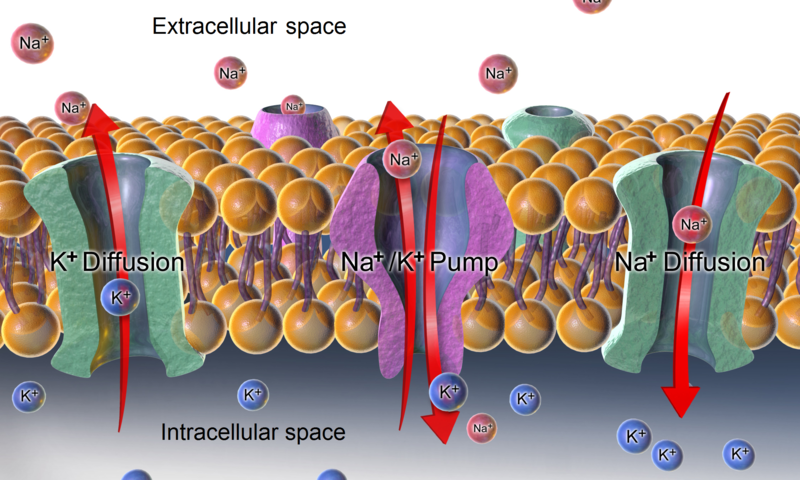
\includegraphics[width=\tmpwidth]{Sodium-potassium_pump_and_diffusion.png} & %
			\onslide<3->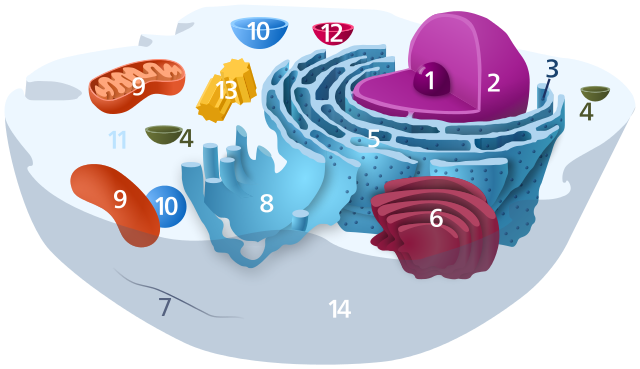
\includegraphics[width=\tmpwidth]{640px-Animal_Cell-svg.png} & % 
			\onslide<4->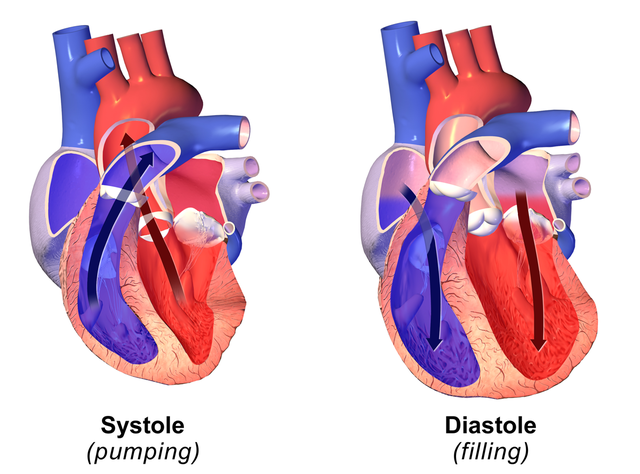
\includegraphics[width=\tmpwidth]{Systolevs_Diastole.png}
		\end{tabular}
	\end{table}
	
	\vfill \hfill \hyperlink{geneontology}{\beamerreturnbutton{go back}}
	
\end{frame}


\begin{frame}[label=aphylo-goexample]
\frametitle{The Gene Ontology Project}

Example of GO term

\begin{table}
\footnotesize
\begin{tabular}{lm{.6\linewidth}}
\toprule
\textbf{Accession} & GO:0060047 \\
\textbf{Name} & heart contraction \\
\textbf{Ontology} & biological\_process \\
\textbf{Synonyms} & heart beating, cardiac contraction, hemolymph circulation \\
\textbf{Alternate} & IDs None \\
\textbf{Definition} & The multicellular organismal process in which the heart decreases in volume in a 
characteristic way to propel blood through the body. Source: GOC:dph \\
\bottomrule
\end{tabular}
\caption{Heart Contraction Function. source: \href{http://amigo.geneontology.org/amigo/term/GO:0060047}{amigo.geneontology.org}}
\end{table}%\pause

You know what is interesting about this function?

\vfill \hfill \hyperlink{geneontology}{\beamerreturnbutton{go back}}

\end{frame}

% ------------------------------------------------------------------------------
\begin{frame}[t]

These four species have a gene with that function... \uncover<2->{and two of %
these are part of the same evolutionary tree!}

\vfill

\def\tmpwidth{.30\linewidth}
\begin{table}
\footnotesize
\mode<beamer>{
\begin{tabular}{*{2}{m{\tmpwidth}<\centering}}
\only<1>{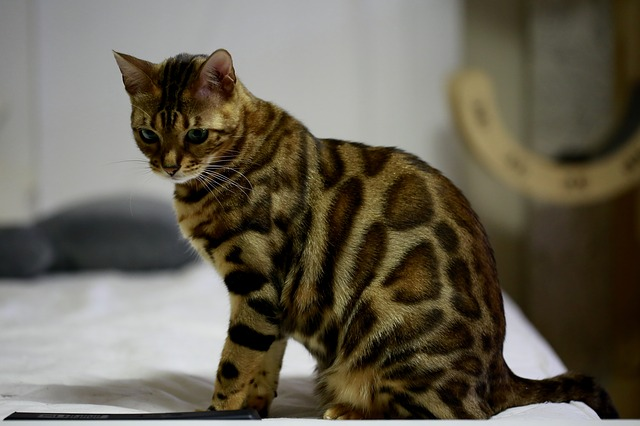
\includegraphics[width=.95\linewidth]{cat.jpg}} %
  \only<2->{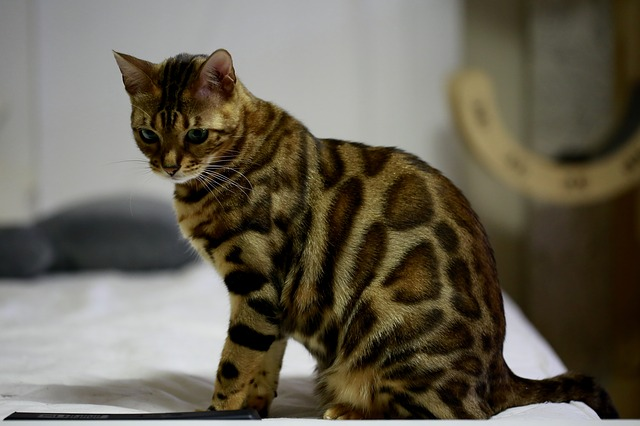
\includegraphics[width=.4\linewidth]{cat.jpg}} \linebreak Felis catus pthr10037 & %
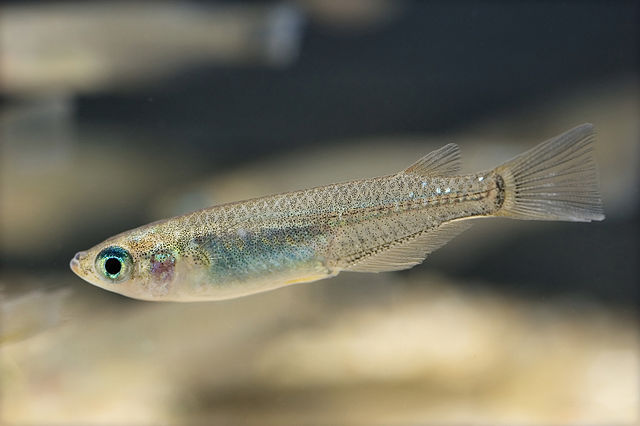
\includegraphics[width=1\linewidth]{Oryzias_latipes.jpg} \linebreak Oryzias latipes \textbf{pthr11521} \\ %
\includegraphics[width=1\linewidth]{Anole_Lizard.jpg} \linebreak Anolis carolinensis \textbf{pthr11521} & %
\only<1>{\includegraphics[width=.725\linewidth]{horse.jpg}} %
  \only<2->{\includegraphics[width=.4\linewidth]{horse.jpg}} \linebreak Equus caballus pthr24356
\end{tabular}
}
\mode<handout>{
	\begin{tabular}{*{2}{m{\tmpwidth}<\centering}}
		\includegraphics[width=.4\linewidth]{cat.jpg} \linebreak Felis catus pthr10037 & %
		\includegraphics[width=1\linewidth]{Oryzias_latipes.jpg} \linebreak Oryzias latipes \textbf{pthr11521} \\ %
		\includegraphics[width=1\linewidth]{Anole_Lizard.jpg} \linebreak Anolis carolinensis \textbf{pthr11521} & %
		\includegraphics[width=.4\linewidth]{horse.jpg} \linebreak Equus caballus pthr24356
	\end{tabular}
}
\end{table}

\vfill \hfill \hyperlink{geneontology}{\beamerreturnbutton{go back}}

\end{frame}

%--------------------------------------------------------------------------------
%\newcommand{\oinclude}[2]{\only<#1>{\includegraphics[width=\tmpwdth,clip,trim={0 0 0 2cm}]{#2}}}

\begin{frame}[t, label=aphylo-good-details]
	\frametitle{Example of Data + Predictions}
	
	\begin{minipage}[m]{.3\linewidth}
		\small
		%	The AUC for this analysis is 0.91 and the Mean Absolute Error is 0.34
		\uncover<1->{\textbf{Family: PTHR11258}}\\
		\uncover<1->{%
			\textbf{Type:} Molecular Function\\
			\textbf{Name:} 2'-5'-oligoadenylate synthetase activity\\
			\textbf{Desc:}  \href{http://amigo.geneontology.org/amigo/term/GO:0001730}{\alert{GO:0001730}} involved in the process of cellular antiviral activity (wiki on \href{https://en.wikipedia.org/wiki/Interferon}{\alert{interferon}}).
		}\\
		\uncover<2->{%
			\textbf{MAE:} 0.34 \\
			\textbf{AUC:} 0.91%
		}
		\vfill
		\hyperlink{aphylo-bad}{\beamerbutton{see a bad one}} 
		\hyperlink{aphylo-good}{\beamerreturnbutton{go back}}
	\end{minipage}
	\begin{minipage}[m]{.65\linewidth}
		\def\tmpwdth{.9\linewidth}
		\mode<beamer>{
			\centering
			\oinclude{1}{example-trees-good1-loo-annotated-parts-1.pdf}%
			\oinclude{2}{example-trees-good1-loo-annotated-0.pdf}%
			\oinclude{3}{example-trees-good1-loo-annotated-1.pdf}%
			\oinclude{4}{example-trees-good1-loo-annotated-2.pdf}%
			\oinclude{5}{example-trees-good1-loo-annotated.pdf}
			%			\only<1>{\includegraphics[width=\tmpwdth, clip, trim={0 0 0 2cm}]{example-trees-good1-loo-annotated-0.pdf}}\only<2>{\includegraphics[width=\tmpwdth, clip, trim={0 0 0 2cm}]{example-trees-good1-loo-annotated-1.pdf}}\only<3>{\includegraphics[width=\tmpwdth, clip, trim={0 0 0 2cm}]{example-trees-good1-loo-annotated-2.pdf}}\only<4>{\includegraphics[width=\tmpwdth, clip, trim={0 0 0 2cm}]{example-trees-good1-loo-annotated.pdf}}
		}
		
		\mode<handout>{
			\centering
			\includegraphics[width=\tmpwdth, clip, trim={0 0 0 2cm}]{example-trees-good1-loo-annotated.pdf}
		}
		
	\end{minipage}
\end{frame}

\begin{frame}[t,label=aphylo-bad]
	\frametitle{Example 2: Bad quality prediction}
	
	\begin{minipage}[m]{.3\linewidth}
		\small
		%	The AUC for this analysis is 0.91 and the Mean Absolute Error is 0.34
		\textbf{MAE:} 0.52 \\
		\textbf{AUC:} 0.33 \\
		\textbf{Type:} Molecular Function\\
		\textbf{Name:} mannosyl-oligosaccharide 1,2-alpha-mannosidase activity\\
		\textbf{Desc:}  \href{http://amigo.geneontology.org/amigo/term/GO:0004571}{\alert{GO:0004571}} involved in synthesis of glycoproteins (\href{https://en.wikipedia.org/wiki/Mannosyl-oligosaccharide_1,2-alpha-mannosidase}{\alert{wiki}} and \href{https://en.wikipedia.org/wiki/Glycoprotein}{\alert{examples}}).
		
		\hyperlink{aphylo-good}{\beamerreturnbutton{go back}}
	\end{minipage}
	\begin{minipage}[m]{.65\linewidth}
		\def\tmpwdth{.9\linewidth}
		\mode<beamer>{
			\centering
			\only<1>{\includegraphics[width=\tmpwdth, clip, trim={0 0 0 2cm}]{example-trees-bad1-loo-annotated-0.pdf}}\only<2>{\includegraphics[width=\tmpwdth, clip, trim={0 0 0 2cm}]{example-trees-bad1-loo-annotated-1.pdf}}\only<3>{\includegraphics[width=\tmpwdth, clip, trim={0 0 0 2cm}]{example-trees-bad1-loo-annotated.pdf}}
		}
		
		\mode<handout>{
			\centering
			\includegraphics[width=\tmpwdth, clip, trim={0 0 0 2cm}]{example-trees-bad1-loo-annotated.pdf}
		}
		
	\end{minipage}
	
	
\end{frame}


%% ------------------------------------------------------------------------------
%\begin{frame}[label=other-models]
%\frametitle{Predicting gene functions}
%There are various approaches for this, some to highlight
%\begin{itemize}%[<+->]
%\item Text analysis like in \cite{Pesaranghader2016}
%\item Protein-protein interaction networks like in \cite{Oliver2000,Piovesan2015}.
%\item Phylogenetic based like SIFTER \cite{Engelhardt2005,Engelhardt2011}.
%\begin{itemize}
%\item Parameters to estimate: $2^{2P}$, where $P$ is the number of functions.
%\end{itemize}
%\end{itemize}
%
%\vfill \hfill (a nice literature review in \cite{Jiang2016,Yu2018})
%\hyperlink{aphylographicalview}{\beamerreturnbutton{go back}}
%
%\end{frame}


% ------------------------------------------------------------------------------
%\begin{frame}[label=aphyloalgorithmicview]
%\frametitle{An evolutionary model of gene functions (algorithmic view)}
%
%\scalebox{.7}{
%
%\begin{algorithm}[H]
%\SetAlgoLined
%\KwData{A phylogenetic tree, $\{\pi, \mu, \psi\}$(Model probabilities)}
%\KwResult{An annotated tree}
%%\pause
%\For{$n \in PostOrder(N)$}{
%  $\mbox{\bf\color{usccardinal}Nodes gain/loss function depending on their parent}$\;%\pause
%  \Switch{class of $n$}{
%    \uCase{root node}{
%      Gain function with probability $\pi$\;
%    }%\pause
%    \uCase{interior node} {%\pause
%      \lIf{Parent has the function}{Keep it with prob. $(1-\mu_1)$}%\pause
%      \lElse{Gain it with prob. $\mu_0$}%\pause
%    }
%  }%\pause
%  $\mbox{\bf\color{usccardinal}Finally, we allow for mislabeling}$\;%\pause
%  \uIf{$n$ is leaf}{%\pause
%    \lIf{has the function}{Mislabel with prob. $\psi_1$}%\pause
%    \lElse{Mislabel with prob. $\psi_0$}%\pause
%  }
%}
%\end{algorithm}
%}
%
%\vfill\hfill \hyperlink{aphylographicalview}{\beamergotobutton{go back}}
%
%
%\end{frame}

% --------------------------
\begin{frame}[label=aphylo-pooled]

% latex table generated in R 3.6.3 by xtable 1.8-4 package
% Tue Apr 28 11:51:17 2020
\begin{table}[tb]
	\centering
	\begin{tabular}{m{.14\linewidth}*{3}{m{.14\linewidth}<\centering}}
		\toprule & \multicolumn{1}{c}{\textit{Pooled-data}} & \multicolumn{2}{c}{One-at-a-time} \\ \cmidrule(r){2-2}\cmidrule(r){3-4}
		& Beta prior & Unif. prior & Beta Prior \\ 
		\midrule
		\textit{Pooled-data} \\
		\hspace{2mm}Unif. prior & \cellcolor{blue!25}[-0.02,-0.01] & \cellcolor{blue!25}[-0.14,-0.10] & \cellcolor{blue!25}[-0.06,-0.03] \\ 
		\hspace{2mm}Beta prior &  - & \cellcolor{blue!25}[-0.12,-0.09] & \cellcolor{blue!25}[-0.04,-0.01] \\ 
		\textit{One-at-a-time} \\
		\hspace{2mm}Unif. prior &  - & - & \cellcolor{red!25}[\hphantom{-}0.06,\hphantom{-}0.09] \\ 
		\bottomrule
	\end{tabular}
	\caption[Differences in Mean Absolute Error]{Differences in Mean Absolute Error [MAE]. Each cell shows the 95\% confidence interval for the difference in MAE resulting from two methods (row method minus column method). Cells are color coded blue when the method on that row has a significantly smaller MAE than the method on that column; Conversely, cells are colored red when the method in that column outperforms the method in that row.  Overall, predictions calculated using the parameter estimates from \textit{pooled-data} predictions outperform \textit{one-at-a-time}.}
	\label{tab:vs-accuracy}
\end{table}

\end{frame}

% ------------------------------------------------------------------------------
\begin{frame}[label=aphylographicalview-altview,c]
	\frametitle{An evolutionary model of gene functions}
	\def\shadowsize{2pt}
	\definecolor{rootnode}{RGB}{0,159,211}
	\definecolor{innernode}{RGB}{90,159,89}
	\definecolor{leafnode}{RGB}{255,107,0}
	
	\begin{minipage}[m]{.60\linewidth}
		\begin{figure}
			\footnotesize
			\centering
			\def\svgwidth{.9\linewidth}
			\mode<beamer>{
				\only<1>{\input{fig/phylo-model-0.pdf_tex}}%
				\only<2>{\input{fig/phylo-model-0b.pdf_tex}}%
				\only<3>{\input{fig/phylo-model-0c.pdf_tex}}%
				\only<4>{\input{fig/phylo-model-1.pdf_tex}}%
				\only<5-6>{\input{fig/phylo-model-2a.pdf_tex}}%
				\only<7>{\input{fig/phylo-model-2b.pdf_tex}}%
				\only<8>{\input{fig/phylo-model.pdf_tex}}
			}\mode<handout>{\input{fig/phylo-model.pdf_tex}}
		\end{figure}
	\end{minipage}
	\hfill
	\begin{minipage}[m]{.38\linewidth}
		\pause
		\begin{itemize}
			\item \textcolor{rootnode}{Root has the function.}\pause[4]
			\item \textcolor{innernode}{Gain\pause{} and loss\pause{} (also depends on the type of event \hyperlink{duplicationvsspeciation}{\beamergotobutton{more}}}).\pause
			\item \textcolor{leafnode}{\textbf{Observed} annotations may be incorrect.}\pause
			\item Only a fraction of the known genes have some form of annotation.
		\end{itemize}
		\vfill\hfill\hyperlink{aphylographicalview}{\beamerreturnbutton{go back}}
	\end{minipage}
	
\end{frame}


% ------------------------------------------------------------------------------
\begin{frame}[label = duplicationvsspeciation]
\frametitle{Speciation}
\begin{figure}
\centering
\def\svgwidth{.8\linewidth}
\tiny
% Source 
\input{fig/Drosophila_speciation_experiment.pdf_tex}
\caption{\cite{Dodd1989}: After one year of isolation, flies showed a significant level of assortativity in mating (\href{https://commons.wikimedia.org/wiki/File:Drosophila_speciation_experiment.svg}{wikimedia})}
\end{figure}

\vfill\hfill \hyperlink{aphylographicalview}{\beamerreturnbutton{go back}}

\end{frame}

\begin{frame}
\frametitle{Duplication}
\begin{figure}
\centering
\def\svgwidth{.6\linewidth}
\tiny
% Source : https://en.wikipedia.org/wiki/File:Evolution_fate_duplicate_genes_-_vector.svg
\input{fig/Evolution_fate_duplicate_genes_-_vector.pdf_tex}
\caption{A key part of molecular innovation, gene duplication provides opportunity for new functions to emerge (\href{https://en.wikipedia.org/wiki/File:Evolution_fate_duplicate_genes_-_vector.svg}{wikimedia})}
\end{figure}

\vfill\hfill \hyperlink{aphylographicalview}{\beamerreturnbutton{go back}}

\end{frame}

% ------------------------------------------------------------------------------
\begin{frame}[label=aphylo-data]
	\frametitle{Data: Phylogenetic trees}
	
	Sample of annotations (first 10 in a single tree, Phosphoserine Phosphatase [PTHR10000])
	
	\small
	
	\begin{table}[ht]
		\centering
		\begin{tabular}{rrll}
			\toprule
			Internal id & Branch Length & type & ancestor \\ 
			\midrule
			AN0 &  & S & LUCA \\ 
			AN1 & 0.06 & S & Archaea-Eukaryota \\ 
			AN2 & 0.24 & S & Eukaryota \\ 
			AN3 & 0.44 & S & Unikonts \\ 
			AN4 & 0.42 & S & Opisthokonts \\ 
			AN6 & 0.68 & D &  \\ 
			AN9 & 0.79 & S & Amoebozoa \\ 
			AN10 & 0.18 & D &  \\ 
			AN15 & 0.57 & S & Dictyostelium \\ 
			AN18 & 0.52 & S & Alveolata-Stramenopiles \\ 
			\bottomrule
		\end{tabular}
	\end{table}
	\vfill\hfill\hyperlink{phylo-table}{\beamerreturnbutton{go back}}
\end{frame}

\begin{frame}
	\frametitle{Data: Node type (events)}
	\begin{figure}
		\centering
		\includegraphics[width=.7\linewidth]{distribution-event-type.pdf}
	\end{figure}
	\vfill\hfill\hyperlink{phylo-table}{\beamerreturnbutton{go back}}
\end{frame}

\begin{frame}
	\frametitle{Data: Annotations (example)}
	
	This is the first 10 of $\sim$ 400,000 experimental annotations used:
	
	\footnotesize
	\begin{table}[ht]
		\centering
		\begin{tabular}{rllll}
			\toprule
			& Family & Id & GO term & Qualifier \\ 
			\midrule
			1 & PTHR12345 & HUMAN$|$HGNC=15756$|$UniProtKB=Q9H190 & GO:0005546 &  \\ 
			2 & PTHR11361 & HUMAN$|$HGNC=7325$|$UniProtKB=P43246 & GO:0016887 & CONTRIBUTES\_TO \\ 
			3 & PTHR10782 & MOUSE$|$MGI=MGI=3040693$|$UniProtKB=Q6P1E1 & GO:0045582 &  \\ 
			4 & PTHR23086 & ARATH$|$TAIR=AT3G09920$|$UniProtKB=Q8L850 & GO:0006520 &  \\ 
			5 & PTHR32061 & RAT$|$RGD=619819$|$UniProtKB=Q9EPI6 & GO:0043197 &  \\ 
			6 & PTHR46870 & ARATH$|$TAIR=AT3G46870$|$UniProtKB=Q9STF9 & GO:1990825 &  \\ 
			7 & PTHR15204 & MOUSE$|$MGI=MGI=1919439$|$UniProtKB=Q9Z1R2 & GO:0045861 &  \\ 
			8 & PTHR22928 & DROME$|$FlyBase=FBgn0050085$|$UniProtKB=Q9XZ34 & GO:0030174 &  \\ 
			9 & PTHR35972 & HUMAN$|$HGNC=34401$|$UniProtKB=A2RU48 & GO:0005515 &  \\ 
			10 & PTHR10133 & DROME$|$FlyBase=FBgn0002905$|$UniProtKB=O18475 & GO:0097681 &  \\ 
			\bottomrule
		\end{tabular}
	\end{table}
	\vfill\hfill\hyperlink{phylo-table}{\beamerreturnbutton{go back}}
\end{frame}

\begin{frame}
	\frametitle{Data: Experimental Annotations}
	\begin{figure}
		\centering
		\includegraphics[width=.7\linewidth]{distribution-annotation-type.pdf}
	\end{figure}
	\vfill\hfill\hyperlink{phylo-table}{\beamerreturnbutton{go back}}
\end{frame}

\begin{frame}[label=aphylo-results-overview]
	\frametitle{Results: Implementation and Large scale study}
	
	\begin{minipage}[m]{.69\linewidth}
		\begin{itemize}
			\item<1-> Simulation, estimation, and prediction: \textbf{aphylo} R package.
			\item<2-> Large simulation study (all known trees, about 15,000) on USC's HPC cluster.
			\item<3-> Prediction quality assessment on $\sim$ 1,300 genes involving $\sim$ 130 families...
			estimation of parameters using a pooled-data model ($<$ 5 min). \hyperlink{aphylo-model-levels}{\beamerreturnbutton{modeling}} \hyperlink{aphylo-table}{\beamerreturnbutton{estimates}}
			\item<4-> In a subset of $\sim 200$ predictions we found 46 novel annotations 
			\hyperlink{aphylo-200funs}{\beamergotobutton{more}}
		\end{itemize}
	\end{minipage}\hfill
	\begin{minipage}[m]{.3\linewidth}
		\begin{center}
			\includegraphics[width=.9\linewidth]{aphylo-logo.png}
		\end{center}
	\end{minipage}
	
	\vfill\hfill\hyperlink{aphylo-results-brief}{\beamerreturnbutton{go back}}
	
\end{frame}

\begin{frame}[c]
	\frametitle{Results: Performance and Scalability}
	aphylo vs SIFTER (state-of-the-art phylo-based model) on 147 genes.
	
	\begin{minipage}[m]{.50\linewidth}
		\bigskip
		\uncover<3->{\begin{figure}
				\includegraphics[width=1\linewidth]{auc.pdf}
		\end{figure}}
	\end{minipage}\hfill
	\begin{minipage}[m]{.45\linewidth}
		\bigskip
		\begin{itemize}
			\item<2->[] \shadowbox{Fast} 110 minutes (SIFTER) to calculate the posterior probabilities, aphylo took 1 second.
			\item<3->[] \shadowbox{Accurate} aphylo reported higher accuracy levels in LOO cross-validation (0.72 vs 0.60 AUC).
		\end{itemize}
	\end{minipage}
	
\end{frame}

% ------------------------------------------------------------------------------
\begin{frame}[c, label=aphylo-model-levels]
	\frametitle{Phylogenetics Modeling: Pooling data}
	
	\begin{minipage}[m]{.5\linewidth}
		\begin{figure}
			\mode<beamer>{
				\includegraphics<1-2>[width=.8\linewidth]{phylo-bayes-a.pdf}%
				\includegraphics<3>[width=.8\linewidth]{phylo-bayes-b.pdf}%
				\includegraphics<4>[width=.8\linewidth]{phylo-bayes-c.pdf}%
				\includegraphics<5->[width=.8\linewidth]{phylo-bayes.pdf}
			}%
			\mode<handout>{\includegraphics<5>[width=.8\linewidth]{phylo-bayes.pdf}}
		\end{figure}
	\end{minipage}
	\begin{minipage}[m]{.48\linewidth}
		\begin{enumerate}
			\item[(a)]<2-> Featured in the first version of the model.
			\item[(b)]<3-> ``Full glory'' Hierarchical Bayes (1,001 parameters for the 141 functions).
			\item[(c)]<4-> Distilled version (a), improves accuracy.
			\item[(d)]<5-> Model estimated for Molecular Function (using Empirical Bayes) without significant improvements.
		\end{enumerate}
	\end{minipage}
	\vfill
	\uncover<6->{All methods are now available in the \texttt{aphylo} package: \texttt{aphylo\_mle}, \texttt{aphylo\_mcmc}, and \texttt{aphylo\_hier}.}
	
	\hyperlink{aphylo-results-overview}{\beamerreturnbutton{go back}}
	
\end{frame}


% ------------------------------------------------------------------------------
% ------------------------------------------------------------------------------
% ------------------------------------------------------------------------------
% ------------------------------------------------------------------------------


\begin{frame}[c,label=aphylo-table]
	\frametitle{Overview of Prediction Results}
	
	\begin{minipage}[m]{.55\linewidth}
		\begin{table}
			\centering
			\scalebox{.64}{
				\begin{tabular}{%
						m{.24\linewidth}<\raggedright %
						>{\color<1>{usccardinal}}m{.24\linewidth}<\centering%
						>{\color<2>{usccardinal}}m{.24\linewidth}<\centering%
						>{\color<3>{usccardinal}}m{.24\linewidth}<\centering%
						>{\color<4>{usccardinal}}m{.24\linewidth}<\centering}
					\toprule
					& & \multicolumn{3}{c}{Type of Annotation} \\
					\cmidrule(r){3-5} %
					\phantom{\LARGE Cellular Component}& %
					\alt<1>{\LARGE Pooled}{Pooled} & %
					\alt<2>{\LARGE Molecular Function}{Molecular Function} & %
					\alt<3>{\LARGE Biological Process}{Biological Process} & %
					\alt<4>{\LARGE Cellular Comp.}{Cellular Component} \\ 
					\midrule
					\multicolumn{3}{l}{\hspace{-10pt}Mislabeling} \\
					$\psi_{01}$ & 0.23 & 0.18 & 0.09 & \multirow{11}{*}{\uncover<4->{\Huge ?}}\\ %0.66 \\ 
					$\psi_{10}$ & 0.01 & 0.01 & 0.01 & \\ %0.33 \\ 
					\multicolumn{3}{l}{\hspace{-10pt}Duplication Events} \\
					$\mu_{d01}$ & 0.97 & 0.97 & \hlcAlt{3}{0.10} & \\ %0.55 \\ 
					$\mu_{d10}$ & 0.52 & 0.51 & \hlcAlt{3}{0.03} & \\ %0.56 \\ 
					\multicolumn{3}{l}{\hspace{-10pt}Speciation Events} \\
					$\mu_{s01}$ & 0.05 & 0.05 & 0.05 & \\ % 0.37 \\ 
					$\mu_{s10}$ & 0.01 & 0.01 & 0.02 & \\ % 0.37 \\ 
					\multicolumn{3}{l}{\hspace{-10pt}Root node} \\
					$\pi$ & 0.79 & 0.71 & 0.88 & \\ %0.52 \\ \midrule
					Trees & 141 & 74 & 45 & 22 \\ 
					\multicolumn{3}{l}{\hspace{-10pt}Accuracy under the by-aspect model} \\
					AUC & - & \hlcAlt{2}{0.77} & \hlcAlt{3}{0.83} & \\ % 0.53 \\ 
					MAE & - & \hlcAlt{2}{0.34} & \hlcAlt{3}{0.26} & \\ % 0.50 \\ 
					\multicolumn{3}{l}{\hspace{-10pt}Accuracy under the pooled-data model} \\
					AUC & - & \hlcAlt{2}{0.77} & 0.75 & \\ % 0.75 \\ 
					MAE & - & \hlcAlt{2}{0.35} & 0.34 & \\ %0.37 \\ 
					\bottomrule
			\end{tabular}}
			%\caption[Parameter estimates comparing pooled-data vs by-type]{MCMC estimates for experimentally annotated trees. The first column shows the estimates under the pooled-data model in \ref{tab:pooled-experimentally-annotated}, while the following three columns report the estimates obtained when fitting the model using a pooled-data approach, but doing so by type of annotation. Readers should be aware that the estimation process of the fourth column, \textit{cellular component}, did not fully converge, likely due to sparsity of annotations within that category.}
			\label{tab:by-aspect-estimates}
		\end{table}
	\end{minipage}
	\hfill
	\begin{minipage}[m]{.44\linewidth}
		Previously, joint estimates out-performed one-at-a-time\pause
		\begin{itemize}
			\item \textbf{Molecular Function} No change.\pause
			\item \textbf{Biological Process} Significantly better.\pause
			\item \textbf{Cellular Component} Does not converge.\pause
		\end{itemize}
		
		
		
		\small
		\begin{table}
			\begin{tabular}{%
					m{.22\linewidth}<\centering m{.03\linewidth}<\centering%
					m{.22\linewidth}<\centering m{.03\linewidth}<\centering%
					m{.25\linewidth}<\centering%
				}
				Molecular Function & $\neq$ & Biological Process &  ? & Cellular Component
			\end{tabular}
		\end{table}
		\normalsize
		
		\only<1->{\vfill\hfill\hyperlink{phylo-data}{\beamergotobutton{data}}}
		\only<1->{\vfill\hfill\hyperlink{aphylo-results-overview}{\beamergotobutton{go back}}}
		
	\end{minipage}
	
	
	
\end{frame}

\begin{frame}[c,label=aphylo-200funs]
	\begin{figure}
		\includegraphics[width=.6\linewidth]{aphylo-results.pdf}
		\caption{Distribution of predictions}
	\end{figure}
	\vfill\hfill\hyperlink{aphylo-results-overview}{\beamerreturnbutton{go back}}
\end{frame}

%-------------------------------------------------------------------------------
\begin{frame}[label=discrete-exponential-theory]
	\frametitle{Asymptotic Behavior of ERGMs}
	
	\begin{itemize}
		\item In the case that $s_l = \s{\graph, x}$ is on the boundary: $s_l \to \pm\infty$\pause
		\item Since the support space of $\s{\graph, x}\in\SUFF$ is bounded, e.g. \# edges $\in [0,n\times (n - 1)]$, we have: \pause
		
		\begin{equation*}
		\lim_{\theta_l\to\infty}\loglik{\theta}, \quad %
		\lim_{\theta_l\to\infty}\nabla\loglik{\theta}, \quad %
		\lim_{\theta_l\to\infty}\mathbf{H}\left(\theta\right)
		\end{equation*}
		log-likelihood, its gradient, and hessian are finite.\pause
		\item The direct implication is that, while $\s{\graph, x}$ is on the boundary, the MLE for the other statistics exists.\footnote{\cite{Handcock2003} briefly mentions this}\pause
		\item All equations ultimately involve realizations of $\s{\graph', x}$ that equal $s_l$, relevant in: Simulations, Bootstrapping, etc.
	\end{itemize}
	
	\vfill\hfill\hyperlink{discrete-exponential}{\beamerreturnbutton{go back}}
	
\end{frame}

%-------------------------------------------------------------------------------
\begin{frame}
	\frametitle{Conditional Graph Distributions}
	
	\begin{itemize}
		\item Long history in (soc.) network science.\pause
		\item Common usage: Hypothesis test prevalence of a feature.\pause{}
		\begin{center}\it
			Is the observed count of XYZ within the expected in a \alert{Bernoulli graph}? \\ \pause{}
			Are statistics A, B, and C different from \alert{graphs with 5 triangles}?
		\end{center}
		\item Different names, same thing, e.g. CUG tests and rewiring algorithms.\pause
		\item $\{\mbox{CUG}, \mbox{Rewiring}\}\subset \mbox{ERGM}$\pause
		\item We can talk about \textit{Conditional} ERGMs.
		
		\begin{equation*}
		\Prcond{\sufstats{\Graph}_k = s_k}{\sufstats{\Graph}_l = s_l, \theta} = %
		\frac{%
			\exp{\transpose{\theta}_{-l}\sufstats{\graph}_{-l}}
		}{%
			\sum_{\graph': \sufstats{\graph'}_l = \sufstats{\graph}_l}\exp{\transpose{\theta}_{-l}\sufstats{\graph'}_{-l}}
		}%\tag{Eq in 3.5 thesis}
		\end{equation*}
		\pause In this equation $\theta_l$ becomes a nuisance parameter.
		
		
	\end{itemize}
	
	\vfill\hfill\hyperlink{discrete-exponential}{\beamerreturnbutton{go back}}
	
\end{frame}

% ------------------------------------------------------------------------------
\begin{frame}[label=ergm-terms]
	
	{\bf\color{suffstat} Sufficient statistics} have various forms
	\def\fig1width{.4\linewidth}
	\begin{figure}[!htbp]
		\small
		\centering
		\begin{tabular}{m{.2\linewidth}<\centering m{.4\linewidth}<\raggedright}
			\toprule Representation & Description  \\ \midrule
			\includegraphics[width=\fig1width]{mutual.pdf} & Mutual Ties (Reciprocity)\linebreak[4]$\sum_{i\neq j}y_{ij}y_{ji}$  \\
			\includegraphics[width=\fig1width]{ttriad.pdf} & Transitive Triad (Balance)\linebreak[4]$\sum_{i\neq j\neq k}y_{ij}y_{jk}y_{ik}$  \\
			\includegraphics[width=\fig1width]{homophily.pdf} & Homophily\linebreak[4]$\sum_{i\neq j}y_{ij}\mathbf{1}\left(x_i=x_j\right)$ \\
			\includegraphics[width=\fig1width]{nodeicov2.pdf} & Attribute-receiver effect \linebreak[4]$\sum_{i\neq j}y_{ij}x_j$ \\
			\includegraphics[width=\fig1width]{fourcycle.pdf} & Four Cycle\linebreak[4]$\sum_{i\neq j \neq k \neq l}y_{ij}y_{jk}y_{kl}y_{li}$  \\
			\bottomrule
		\end{tabular}
		\caption[Example of Graph Sufficient Statistics]{Besides the common edge count statistic (number of ties in a graph), ERGMs allow measuring other more complex structures that can be captured as sufficient statistics. }
		\label{fig:ergm-structs}
		\normalsize
	\end{figure}
	
	\vfill\hfill \hyperlink{discrete-exponential}{\beamerreturnbutton{go back}}
\end{frame}

% Simulation study -------------------------------------------------------------

\begin{frame}[t,label=ergmito-simulations]
	\frametitle{Simulation Study}
	
	\begin{minipage}[t]{.3\linewidth}
		\begin{enumerate}
			\item \alert{\bf Higher convergence rate}
		\end{enumerate}
		\vfill\hyperlink{ergmito-results-brief}{\beamerreturnbutton{return}}
	\end{minipage}
	\vfill\hfill\begin{minipage}[t]{.65\linewidth}\vspace{-.75cm}
		\begin{figure}
			\centering
			\includegraphics[width=.9\linewidth]{failed.pdf}
		\end{figure}
	\end{minipage}
\end{frame}

\begin{frame}[t, label=ergmitoexperiment]
	\frametitle{Simulation Study}
	
	\begin{minipage}[t]{.3\linewidth}
		\begin{enumerate}
			\item Higher convergence rate
			\item \alert{\bf Smaller bias}
		\end{enumerate}
		\vfill\hyperlink{ergmito-results-brief}{\beamerreturnbutton{return}}
	\end{minipage}
	\vfill\hfill\begin{minipage}[t]{.65\linewidth}\vspace{-.75cm}
		\begin{table}
			\centering
			\begin{tabular}{rccc}
				\toprule
				& MLE & MC-MLE & RM \\ 
				\midrule
				edges & [0.27, 0.36] & [1.23, 1.65] & [0.55, 1.54] \\ 
				ttriads & [-0.05, -0.03] & [-0.22, -0.16] & [-0.15, 0.48] \\ 
				\bottomrule
			\end{tabular}
			\caption[Empirical Biases per Method]{\label{tab:empirical-bias-sim}Empirical bias. Each cell shows the 95\% confidence interval of each methods' empirical bias.} 
		\end{table}
		
		\hfill\hyperlink{ergmito-bias}{\beamergotobutton{alt take}}
	\end{minipage}
\end{frame}

\begin{frame}[t]
	\frametitle{Simulation Study}
	
	\begin{minipage}[t]{.3\linewidth}
		\begin{enumerate}
			\item Higher convergence rate
			\item Smaller bias
			\item \alert{\bf Higher power}
		\end{enumerate}
		\vfill\hyperlink{ergmito-results-brief}{\beamerreturnbutton{return}}
	\end{minipage}
	\hfill\begin{minipage}[t]{.65\linewidth}%\vspace{-.75cm}
		\begin{figure}
			\centering
			%		\caption[Empirical Power by Sample and Effect Size]{\label{fig:power}Empirical power by dataset size and effect size (the later considering only magnitude), for ERGM and \ergmito{} estimation methods. Power increases for both MC-MLE (ERGM) and MLE (\ergmito{}) with increases in the size of the dataset and effect size. There are indistinguishable differences in power between the two estimation methods.}
			\includegraphics[width=.95\linewidth]{power.pdf}
		\end{figure}
	\end{minipage}
\end{frame}

\begin{frame}[t]
	\frametitle{Simulation Study}
	
	\begin{minipage}[t]{.3\linewidth}
		\begin{enumerate}
			\item Higher convergence rate
			\item Smaller bias
			\item Higher power
			\item \alert{\bf Smaller type I error}
		\end{enumerate}
		\vfill\hyperlink{ergmito-results-brief}{\beamerreturnbutton{return}}
	\end{minipage}
	\hfill\begin{minipage}[t]{.65\linewidth}%\vspace{-.75cm}
		\begin{table}
			\centering\small
			\begin{tabular}{*{2}{m{.1\linewidth}<\centering}*{5}{c}}
				\toprule & & \multicolumn{3}{c}{P(Type I error)} & \multicolumn{2}{c}{$\chi^2$ (vs MLE)}\\ \cmidrule(r){3-5} \cmidrule(r){6-7}
				Sample size & N. Sims. & MLE & MC-MLE & RM & MC-MLE & RM \\ 
				\midrule
				5 & 4,325 & 0.066 & 0.086 & 0.086 & 11.36 *** & 11.36 *** \\ 
				10 & 4,677 & 0.063 & 0.078 & 0.073 & 8.44 *** & 3.73 * \\ 
				15 & 4,818 & 0.060 & 0.072 & 0.063 & 5.50 ** & 0.41  \\ 
				20 & 4,889 & 0.054 & 0.065 & 0.061 & 5.30 ** & 2.05  \\ 
				30 & 4,946 & 0.053 & 0.059 & 0.055 & 1.60  & 0.07  \\ 
				50 & 4,987 & 0.053 & 0.055 & 0.047 & 0.16  & 1.67  \\ 
				100 & 4,999 & 0.054 & 0.054 & 0.050 & 0.00  & 0.81  \\ 
				\bottomrule
			\end{tabular}
			%		\caption[Empirical Type I Error Rates]{\label{tab:typeI}Empirical Type I error rates. The $\chi^2$ statistic is from a 2-sample test for equality of proportions, and the significance levels are given by *** $p < 0.01$, ** $p < 0.05$, and * $p < 0.10$.} 
		\end{table}
	\end{minipage}
\end{frame}

\begin{frame}[t]
	\frametitle{Simulation Study}
	
	\begin{minipage}[t]{.3\linewidth}
		\begin{enumerate}
			\item Higher convergence rate
			\item Smaller bias
			\item Higher power
			\item Smaller type I error
			\item \alert{\bf Elapsed time}
		\end{enumerate}
		\vfill\hyperlink{ergmito-results-brief}{\beamerreturnbutton{return}}
	\end{minipage}
	\hfill\begin{minipage}[t]{.65\linewidth}%\vspace{-.75cm}
		\begin{figure}
			\centering
			%	\caption[Distribution of Elapsed Time]{\label{fig:elapsedtime}Distribution of elapsed time (in seconds) for the estimation process for MC-MLE (ERGM) versus MLE (using \ergmito{}). Overall, the MLE implementation is orders of magnitude faster compared to the time required by the MC-MLE implementation to do the parameter estimation.}
			\small
			\def\svgwidth{.9\linewidth}
			\input{fig/time.pdf_tex}
		\end{figure}
	\end{minipage}
\end{frame}

% ------------------------------------------------------------------------------
\begin{frame}[c,label=ergmito-teams-data]
	\frametitle{Featured Application: Small Teams}
	
	\begin{minipage}[t]{.38\linewidth}
		\small
		\noindent \textbf{Sample}
		\pause
		\begin{itemize}
			\item 31 mixed-gender teams (4-5 members).\pause
			\item University students.\pause
			\item Don't know each other.\pause
			\item At least one female/male per team.\pause
		\end{itemize}
		\noindent \textbf{Experiment}\pause
		\begin{itemize}
			\item Complete 1 hour of group tasks.\pause
			\item Captured network data using name generator survey: \textit{Who did you go to for advice, information or help to complete the group task?}
		\end{itemize}
	\end{minipage}
	\hfill
	\begin{minipage}[t]{.6\linewidth}
		\centering
		\uncover<9->{
			\begin{figure}
				\includegraphics[width=.95\linewidth]{ci-ergm-all-nets.pdf}
			\end{figure}
			\uncover<10->{\Large Is Gender Homophily a feature of these graphs?}
		}
	\end{minipage}
	\vfill\hfill\hyperlink{ergmito-applied}{\beamerreturnbutton{go back}}
\end{frame}

%-------------------------------------------------------------------------------
\begin{frame}[label=ergmito-table]
	
	\begin{minipage}[c]{.7\linewidth}
		\begin{table}
			\centering
			\scalebox{.65}{
				\begin{tabular}{l c c c c c c }
					\toprule
					& (1) & (2) & (3) & \hlcAlt{5}{(4)} & (5) & \hlcAlt{5}{(4b)} \\
					\midrule
					edges                                     & $-0.52^{**}$  & $-0.91^{***}$ & $-0.54^{**}$  & $-0.72^{***}$ & $-0.48^{*}$   & $-0.72^{***}$ \\
					& $(0.17)$      & $(0.23)$      & $(0.18)$      & $(0.19)$      & $(0.19)$      & $(0.17)$      \\
					ttriads                                   & $0.36^{***}$  & $0.46^{***}$  & $0.37^{***}$  & $0.36^{***}$  & $0.36^{***}$  & $0.36^{***}$  \\
					& $(0.06)$      & $(0.06)$      & $(0.06)$      & $(0.06)$      & $(0.06)$      & $(0.05)$      \\
					%				\only<3>{\rowcolor{gray!50}} %
					\hlcAlt{6}{Homophily (gender)}                        & $-0.03$       & $-0.01$       & $-0.20$       & $-0.12$       & $-0.01$       & $-0.12$       \\
					& $(0.20)$      & $(0.21)$      & $(0.46)$      & $(0.20)$      & $(0.20)$      & $(0.20)$      \\
					\hlcAlt{2}{$\text{edges} \times \isone{n = 5}$}       & $-0.53^{***}$ & $-0.47^{**}$  & $-0.52^{***}$ & $-0.53^{***}$ & $-0.53^{***}$ & $-0.53^{***}$ \\
					& $(0.12)$      & $(0.16)$      & $(0.13)$      & $(0.13)$      & $(0.12)$      & $(0.13)$      \\
					\hlcAlt{3}{$(\text{Homophily})^{1/2}$}                &               &               & $0.54$        &               &               &               \\
					&               &               & $(1.32)$      &               &               &               \\
					\hlcAlt{6}{Sender (female)}                           &               &               &               & $0.46^{*}$    &               & $0.46^{*}$    \\
					&               &               &               & $(0.18)$      &               & $(0.18)$      \\
					Receiver (female)                           &               &               &               &               & $-0.08$       &               \\
					&               &               &               &               & $(0.18)$      &               \\
					\hlcAlt{4}{\textit{Constraint (offset)}} \\
					\hspace{5mm}$\text{edge} > 4$        &               & Yes        &               &               &               &               \\
					\midrule
					AIC                                       & 639.26        & 569.93        & 641.08        & 634.68        & 641.07        & 634.68        \\
					BIC                                       & 655.99        & 586.66        & 661.99        & 655.59        & 661.98        & 655.59        \\
					Num. networks                             & 31            & 28            & 31            & 31            & 31            & 31            \\
					Time (seconds)                            & 2.26          & 2.32          & 2.28          & 5.10          & 5.19          & 83.97         \\
					N replicates                              &               &               &               &               &               & \hlcAlt{5}{1000}          \\ \bottomrule
					\multicolumn{7}{l}{\scriptsize{$^{***}p<0.001$, $^{**}p<0.01$, $^*p<0.05$}}
			\end{tabular}}
			\label{tab:ci-ergm-full}
		\end{table}
	\end{minipage}
	\hfill
	\begin{minipage}[c]{.28\linewidth}
		\pause\small
		\begin{enumerate}[<+->]
			\item \alert<2>{Interaction effects: seemingly included.}
			\item \alert<3>{Transformed variables: also easy to add.}
			\item \alert<4>{Using offset terms, we can constrain the support.}
			\item \alert<5>{Each 1,000 bootstrap replicates took roughly 0.08 secs.}
			\item \alert<6>{No support for gender homophily, but evidence of females sending more ties.}
		\end{enumerate}
		
		\uncover<7>{What about goodness-of-fit?}
		
	\end{minipage}
	
	
	\vfill\hfill%	
	\hyperlink{ergmito-applied}{\beamerreturnbutton{go back}}
	
\end{frame}


%-------------------------------------------------------------------------------
\begin{frame}[label=ergmito-gof]
	\frametitle{What About Goodness-of-fit?}
	\begin{figure}[!p]
		\centering
		\footnotesize
		\def\svgwidth{.85\linewidth}
		\input{fig/ci-ergmito-gof-full.pdf_tex}
		\label{fig:ci-gof-full}
	\end{figure}
	
	\vfill\hfill\hyperlink{ergmito-applied}{\beamerreturnbutton{go back}}
	
\end{frame}

% ------------------------------------------------------------------------------
\begin{frame}[label=example-data-ergm]
	% latex table generated in R 3.6.3 by xtable 1.8-4 package
	% Mon Apr 27 23:32:51 2020
	\begin{table}
		\centering
		\begin{tabular}{*{3}{c}*{3}{m{.15\linewidth}<\centering}}
			\toprule
			(1) & (2) & (3) & (4) & (5) & (6) \\
			Size ($n$) & edges & ttriads & $\text{edges}\times\isone{n = 5}$ & $\text{ttriads}\times\isone{n = 5}$ & $\text{edges}\times\log{1/n}$ \\ 
			\midrule
			4 &  10 &  14 &   0 &   0 & -13.86 \\ 
			4 &   6 &   2 &   0 &   0 & -8.32 \\ 
			4 &   4 &   0 &   0 &   0 & -5.55 \\ 
			5 &   6 &   1 &   6 &   1 & -9.66 \\ 
			5 &   8 &   8 &   8 &   8 & -12.88 \\ 
			5 &   6 &   2 &   6 &   2 & -9.66 \\ 
			\multicolumn{6}{c}{\dots\textit{25 more rows}\dots} \\
			\bottomrule
		\end{tabular}
		\caption[Example of Observed Sufficient Statistics for the Applied Example]{\label{tab:example-suffstats}Example of observed sufficient statistics for the team advice networks. Pooled-data ERGMs have multiple observed sufficient statistics (also known as target statistics). Furthermore, as shown here, we can manipulate common statistics as \textit{edges} (2) and \textit{ttriads} (3) to include, e.g. interaction effects (4) and (5), or more complex transformations, e.g. (6).}
	\end{table}
\vfill\hfill\hyperlink{ergmito-applied}{\beamerreturnbutton{go back}}
\end{frame}

% ------------------------------------------------------------------------------
\begin{frame}[label=aphylo-current]
	\frametitle{Phylogenetics Modeling Strategies}
	
	\begin{minipage}[m]{.3\linewidth}
		
		\begin{figure}
			\includegraphics[width=.9\linewidth]{phylo-model-overview-legend.pdf}
		\end{figure}
	\end{minipage}\hfill
	\begin{minipage}[m]{.69\linewidth}
		\mode<beamer>{
			\begin{figure}
				\phantom{\includegraphics<1>[width=.9\linewidth]{phylo-model-overview-1.pdf}}%
				\includegraphics<2>[width=.9\linewidth]{phylo-model-overview-1.pdf}%
				\includegraphics<3>[width=.9\linewidth]{phylo-model-overview-2.pdf}%
				\includegraphics<4>[width=.9\linewidth]{phylo-model-overview.pdf}
			\end{figure}
		}
		
		\mode<handout>{
			\begin{figure}
				\includegraphics[width=.9\linewidth]{phylo-model-overview.pdf}
			\end{figure}
		}
	\end{minipage}
	
	\vfill\hfill\hyperlink{current-research}{\beamerreturnbutton{go back}}
	
\end{frame}

% ------------------------------------------------------------------------------
\begin{frame}[c,label=aphylo-ergm-example]
	
	\Large If we wanted to build a model with 3 functions, we would need to estimate...\large
	\\\bigskip
	
	\begin{minipage}[t]{.40\linewidth}
		\centering
		\shadowbox{Full Markov Transition Matrix}\\\bigskip
		\uncover<2->{\includegraphics[width=.8\linewidth]{aphylo-ergm-eq1.png} \\
			\vfill 512 parameters
		}
	\end{minipage}\hfill
	\begin{minipage}[t]{.19\linewidth}
		\centering 
		\uncover<4->{
			\includegraphics[width=.8\linewidth]{aphylo-ergm-eq2.png}\\
			Easier to fit \\
			Easier to interpret}	
	\end{minipage}\hfill
	\begin{minipage}[t]{.40\linewidth}		
		\centering
		\shadowbox{Sufficient statistics}\\\bigskip
		\uncover<3->{\includegraphics[width=.8\linewidth]{aphylo-ergm-eq2.png} \\
			\vfill 5 parameters}
	\end{minipage}
	\uncover<4->{\vfill\hfill\hyperlink{current-research}{\beamerreturnbutton{numeric example}}}
	
\end{frame}


%-------------------------------------------------------------------------------
\begin{frame}[c, label=barry-pkg]
	\frametitle{Barry: your go-to \textit{motif} accountant}
	\centering
	\begin{minipage}[m]{.33\linewidth}
		\small
		\begin{itemize}
			\item<1-> Sparse matrix represented using double hashmaps (fast row/column access).
			\item<2-> Template implementation for flexible weights and metadata.
			%	\item<3-> Full enumeration of array powersets.
			\item<3-> Fast counting using change statistics (\tiny Ch. 4\normalsize).
			\item<4-> Calculation of support for sufficient stats.
		\end{itemize}
		\only<1->{\url{https://USCbiostats.github.io/binaryarrays}}
	\end{minipage}\hfill
	\begin{minipage}[m]{.65\linewidth}
		\begin{figure}
			\begin{minipage}[m]{.49\linewidth}
				\uncover<5->{\includegraphics[width=.99\linewidth]{barray-phylo.png}}
			\end{minipage}
			\begin{minipage}[m]{.49\linewidth}
				\uncover<6->{\includegraphics[width=.99\linewidth]{barray-network.png}}
			\end{minipage}
			\uncover<5->{\caption{Screenshots from the project's website on GitHub.}}
		\end{figure}
	\end{minipage}
\end{frame}


% ------------------------------------------------------------------------------
\begin{frame}[t, label=aphylo-ergm-table]
	\frametitle{What Drives Evolution}
	
	Imagine that we have 3 functions (rows) and that each node has 2 siblings (columns)
	
	\mode<beamer>{
		\begin{table}
			\begin{tabular}{llcc}
				\toprule
				& & \multicolumn{2}{c}{\bf Transitions to} \\
				& & Case 1 & Case 2 \\ \cmidrule(r){3-4}
				\multicolumn{2}{r}{\textbf{Parent} $\begin{array}{c}\mbox{A} \\ \mbox{B} \\ \mbox{C}\end{array}\left[\begin{array}{c}0 \\ 1 \\ 1\end{array}\right]$} & 
				$\left[\begin{array}{cc} %
					0 & \nhlc{1-2}{1}\hlc{3-5}{1}\nhlc{6-}{1} \\ %
					1 & \nhlc{1-3}{0}\hlc{4-5}{0}\nhlc{6-}{0} \\ %
					1 & \nhlc{1-3}{0}\hlc{4}{1}\nhlc{5-}{1} %
				\end{array}\right]$ & 
				$\left[\begin{array}{cc} %
					0 & \nhlc{-2}{1}\nhlc{4}{1}\hlc{3}{1}\hlc{5}{1}\nhlc{6-}{1} \\ %
					\nhlc{-5}{1}\hlc{6}{1} & \nhlc{-4}{0}\hlc{5}{0}\nhlc{6-}{0}\\ %
					\nhlc{-4}{0}\hlc{5}{0}\nhlc{6-}{0} & \nhlc{1-5}{1}\hlc{6}{1}%
				\end{array}\right]$ \pause \\ \midrule 
				\multicolumn{3}{l}{\textbf{Sufficient statistics}} \pause \\ 
				& \# Gains & 1 & 1 \pause \\
				& Only one offspring changes (yes/no) & 1 & 0 \pause \\
				& \# Changes (gain+loss) & 2 & 3 \pause \\
				& Subfunctionalization (yes/no) & 0 & 1 \\ \bottomrule
			\end{tabular}
		\end{table}
	}
	\mode<handout>{
		\begin{table}
			\begin{tabular}{llcc}
				\toprule
				& & \multicolumn{2}{c}{\bf Transitions to} \\
				& & Case 1 & Case 2 \\ \cmidrule(r){3-4}
				\multicolumn{2}{r}{\textbf{Parent} $\begin{array}{c}\mbox{A} \\ \mbox{B} \\ \mbox{C}\end{array}\left[\begin{array}{c}0 \\ 1 \\ 1\end{array}\right]$} & 
				$\left[\begin{array}{cc} %
					0 & 1 \\ %
					1 & 0 \\ %
					1 & 1 %
				\end{array}\right]$ & 
				$\left[\begin{array}{cc} %
					0 & 1 \\ %
					1 & 0\\ %
					0 & 1%
				\end{array}\right]$ \\ \midrule 
				\multicolumn{3}{l}{\textbf{Sufficient statistics}} \\ 
				& \# Gains & 1 & 1  \\
				& Only one offspring changes (yes/no) & 1 & 0 \\
				& \# Changes (gain+loss) & 2 & 3 \\
				& Subfunctionalizations (yes/no) & 0 & 1 \\ \bottomrule
			\end{tabular}
		\end{table}
	}
	
	\vfill\hfill\hyperlink{aphylo-ergm-example}{\beamergotobutton{return}}
	%	\pause
	%	Modeling the full Markov transition matrix would take $2^3 \times 2^6 = 512$ parameters.
	
\end{frame}

%-------------------------------------------------------------------------------
\begin{frame}[c]
	\frametitle{What Drives Evolution: a game changer}
	
	\begin{minipage}[m]{.59\linewidth}
		In the model with 3 functions and 2 offspring per node:\pause
		\begin{itemize}
			\item Full Markov transition matrix: $2^3 \times 2^6 = 512$\pause
			\item Using sufficient statistics:\pause
			\begin{itemize}
				\item[] Pairwise co-evolution: 3 terms,\pause
				\item[]	Pairwise Neofunctionalization: 3 terms,\pause
				\item[] Pairwise Subfunctionalization: 3 terms,\pause
				\item[] Function specific gain: 3 terms,\pause
				\item[] Function specific loss: 3 terms,\pause
				\item[Total:] 15 parameters. \pause
			\end{itemize}
			\item Easier to fit and interpret.
		\end{itemize}
	\end{minipage}\hfill
	\begin{minipage}[m]{.39\linewidth}
		\begin{figure}
			\centering
			\includegraphics[width=.99\linewidth]{phylo-model-overview.pdf}
		\end{figure}
	\end{minipage}
	\vfill\hfill\hyperlink{aphylo-ergm-example}{\beamergotobutton{return}}
\end{frame}

\begin{frame}[allowframebreaks]
	\frametitle{References}
	% \bibliographystyle{apacite}
	% \bibliography{bibliography.bib}
	\printbibliography
\end{frame}

\end{document}

